% !TEX root = saveliev_physics_general_course_2.tex
%!TEX TS-program = pdflatex
%!TEX encoding = UTF-8 Unicode


\chapter[QUANG HỌC]{Quang học}\label{chap:16}
\chaptermark{Quang học}

\section{Sóng ánh sáng}\label{sec:16_1}
\vspace{-12pt}
Ánh sáng là một hiện tượng phức tạp: nó hành xử như một sóng điện từ trong một số trường hợp, và như một dòng các hạt đặc biệt (photon) trong các trường hợp khác. Ở chương này, chúng ta sẽ xem xét quang học sóng, tức là các hiện tượng dựa trên bản chất sóng của ánh sáng. 
Các hiện tượng do bản chất hạt của ánh sáng sẽ được xem xét trong Tập III.


Các vector $\vec{E}$ và $\vec{H}$ là hai thành phần dao động trong một sóng điện từ.
Thực nghiệm cho thấy các tác dụng sinh lý, quang điện, quang hóa và các tác dụng khác của ánh sáng là do sự dao động của thành phần vector điện trường. Do đó sau này khi nói đến \textbf{vector ánh sáng}, tức là ta ám chỉ vector cường độ điện trường. Thành phần từ trường của sóng ánh sáng sẽ không được đề cập đến.


Theo quy ước, ta sẽ kí hiệu biên độ của vector ánh sáng bằng chữ $A$ (hoặc đôi khi bằng kí hiệu $\ab{E}{m}$).
Do đó, sự biến thiên theo không gian và thời gian của hình chiếu của vector ánh sáng lên phương mà vector này dao động sẽ được mô tả bởi phương trình
\begin{equation}\label{eq:16_1}
    E = A \cos(\omega t - kr + \alpha),
\end{equation}

\noindent
trong đó $k$ là số sóng và $r$ là khoảng cách đo theo phương mà sóng ánh sáng lan truyền.

Đối với một sóng phẳng truyền trong một môi trường không hấp thụ, $A = \text{hằng số}$, đối với một sóng cầu, $A$ giảm dần theo tỉ lệ $1/r$.

Tỉ số của vận tốc sóng ánh sáng trong chân không với vận tốc pha $v$ trong một môi trường được gọi là \textbf{chiết suất tuyệt đối} của môi trường đó và được kí hiệu bằng chữ $n$.
Do đó,
\begin{equation}\label{eq:16_2}
    n = \frac{c}{v}.
\end{equation}

\noindent
So sánh với \eqn{15_10} cho thấy $n = \sqrt{\varepsilon\mu}$.
Với phần lớn các chất trong suốt, $\mu$ không sai khác đáng kể so với 1.
Do đó ta có thể coi
\begin{equation}\label{eq:16_3}
    n = \sqrt{\varepsilon}.
\end{equation}

Phương trình \eqref{eq:16_3} liên hệ các tính chất quang và điện của một chất.
Thoạt nhìn thì có vẻ phương trình này không đúng
Ví dụ, với nước $\varepsilon = 81$, trong khi $n = 1.33$.
Tuy nhiên, cần phải nhớ rằng $\varepsilon = 81$ thu được từ những phép đo tĩnh điện.
Một giá trị khác của $\varepsilon$ sẽ thu được từ các điện trường biến đổi nhanh, và giá trị này phụ thuộc vào tần số các dao động của trường.
Điều này giải thích \textbf{sự tán sắc} của ánh sáng, tức là, sự phụ thuộc của chiết suất (hay vận tốc ánh sáng) vào tần số (hay bước sóng).
Thay giá trị $\varepsilon$ thu được ở tần số phù hợp vào \eqn{16_3} sẽ cho ra giá trị đúng của $n$.

Giá trị của chiết suất đặc trưng cho \textbf{mật độ quang học} của môi trường.
Một môi trường có $n$ lớn hơn được gọi là đậm đặc hơn về mặt quang học so với một môi trường có $n$ nhỏ hơn.
Ngược lại, một môi trường có $n$ nhỏ hơn được gọi là ít đậm đặc hơn về mặt quang học so với một môi trường có $n$ nhỏ hơn.

Bước sóng của ánh sáng nhìn thấy được nằm trong khoảng sau:
\begin{equation}\label{eq:16_4}
    \lambda_0 = \text{\SI{0.40}{\micro\metre} đến \SI{0.76}{\micro\metre}} (\text{\SI{4000}{\angstrom} đến \SI{7600}{\angstrom}}).
\end{equation}

\noindent
Các giá trị này là của sóng ánh sáng truyền trong chân không.
Bước sóng của ánh sáng truyền trong các chất khác sẽ có những giá trị khác.
Với sóng ánh sáng dao động với tần số $\nu$, thì bước sóng trong chân không là $\lambda_0 = c/\nu$.
Trong một môi trường mà vận tốc pha của sóng ánh sáng là $v = c/n$, bước sóng có giá trị $\lambda = v/\nu = c/(\nu n) = \lambda_0/n$.
Do đó, độ dài của bước sóng ánh sáng trong một môi trường có chiết suất $n$ được liên hệ với độ dài của bước sóng trong chân không bởi biểu thức
\begin{equation}\label{eq:16_5}
    \lambda = \frac{\lambda_0}{n}.
\end{equation}

Tần số của sóng ánh sáng nhìn thấy được nằm trong khoảng sau:
\begin{equation}\label{eq:16_6}
    \nu = \text{\SI{0.39e15}{\hertz} đến \SI{0.75e15}{\hertz}}.
\end{equation}

\noindent
Tần số biến thiên của mật độ năng thông của sóng sẽ còn lớn hơn (nó bằng $2\nu$).
Mắt chúng ta hay bất kì máy thu quang năng nào cũng đều không thể theo dõi được sự biến thiên năng thông nhanh như vậy, do vậy, những thiết bị đó chỉ ghi nhận được thông lượng trung bình theo thời gian. Độ lớn của vector mật độ năng thông trung bình của một sóng ánh sáng được gọi là \textbf{cường độ sáng} $I$ tại một điểm cho trước trong không gian.
Một độ thông lượng của năng lượng điện từ được xác định bởi vector Poynting $\vec{S}$.
Do đó,
\begin{equation}\label{eq:16_7}
    I = |\average{\vec{S}}| = |\average{\vecprod{E}{H}}|.
\end{equation}

\noindent
Ta lấy trung bình trên khoảng ``thời gian vận hành'' của thiết bị, mà như đã lưu ý ở trên, là lớn hơn rất nhiều so với chu kì dao động của sóng.
Cường độ sáng có thể được đo bằng đơn vị năng lượng (ví dụ, bằng \si{\watt\per\metre\squared}), hoặc bằng đơn vị quang học là ``lumen trên mét vuông'' (xem \sect{16_5}).

Theo \eqn{15_22}, độ lớn biên độ của các vector $\vec{E}$ và $\vec{H}$ trong một sóng điện từ được liên hệ bởi biểu thức
\begin{equation*}
    \ab{E}{m} \sqrt{\varepsilon\varepsilon_0} = \ab{H}{m} \sqrt{\mu\mu_0} = \ab{H}{m} \sqrt{\mu_0}
\end{equation*}

\noindent
(ta đã giả sử rằng $\mu=1$).
Do đó ta có
\begin{equation*}
    \ab{H}{m} = \sqrt{\varepsilon} \parenthesis{\frac{\varepsilon_0}{\mu_0}}^{1/2} \ab{E}{m} = n \ab{E}{m} \parenthesis{\frac{\varepsilon_0}{\mu_0}}^{1/2},
\end{equation*}

\noindent
với $n$ là chiết suất của môi trường mà sóng lan truyền.
Vì vậy, $\ab{H}{m}$ tỉ lệ với $\ab{E}{m}$ và $n$:
\begin{equation}\label{eq:16_8}
    \ab{H}{m} \propto n \ab{E}{m}.
\end{equation}

\noindent
Độ lớn giá trị trung bình của vector Poynting tỉ lệ với $\ab{H}{m}\ab{E}{m}$. Do đó ta có thể viết
\begin{equation}\label{eq:16_9}
    I \propto n \ab{E}{m}^2 = n A^2
\end{equation}

\noindent
(hệ số tỉ lệ là $\sqrt{\varepsilon_0/\mu_0}$).
Như vậy, cường độ sáng tỉ lệ với chiết suất của môi trường và bình phương biên độ sóng ánh sáng.

Cần lưu ý rằng khi xét sự lan truyền của sóng ánh sáng trong một môi trường đồng nhất, ta có thể giả sử rằng cường độ sáng chỉ tỉ lệ với bình phương biên độ sóng
\begin{equation}\label{eq:16_10}
    I \propto A^2.
\end{equation}

\noindent
Tuy nhiên, với ánh sáng truyền qua mặt phân cách giữa các môi trường, thì biểu thức cường độ sáng mà không tính đến thừa số $n$ sẽ dẫn đến sự không bảo toàn quang thông.

Những đường mà trên đó quang năng lan truyền được gọi là \textbf{các tia sáng}.
Vector Poynting trung bình tại mỗi điểm $\average{\vec{S}}$ hướng theo tiếp tuyến với tia sáng tại điểm đó.
Hướng của $\average{\vec{S}}$ trong một môi trường đẳng hướng trùng với một pháp tuyến của mặt sóng, tức là trùng với hướng của vector sóng $\vec{k}$.
Do đó, các tia sáng phải đi vuông góc với các mặt sóng.
Trong một môi trường dị hướng, một pháp tuyến của mặt sóng nói chung là không trùng với hướng của vector Poynting, do đó các tia sáng không đi vuông góc với các mặt sóng.

Mặc dù sóng ánh sáng là sóng ngang, chúng thường không thể hiện sự bất đối xứng đối với một tia sáng.
Có thể giải thích rằng trong ánh sáng \textbf{tự nhiên} (tức là, ánh sáng phát ra từ những nguồn thông thường) có nhiều dao động theo các phương vuông góc với tia sáng (\fig{16_1}).
Sự phát xạ của vật sáng bao gồm các sóng phát ra từ các nguyên tử của nó.
Quá trình phát xạ của một nguyên tử diễn ra trong khoảng \SI{e-8}{\second}.
Trong khoảng thời gian này, một chuỗi các ``nhấp nhô'' (hay một \textbf{đoàn sóng}) có độ dài khoảng ba mét được hình thành.
Các nguyên tử ``ngừng lại'', rồi sau đó lại ``nổi lên'' sau một khoảng thời gian nhất định.
Có nhiều nguyên tử ``nổi lên'' cùng một thời điểm.
Các đoàn sóng mà các nguyên tử phát ra chồng chập với nhau và tạo thành sóng ánh sáng tương đương mà cả vật thể phát ra.
Các mặt phẳng dao động của mỗi đoàn sóng từ các nguyên tử được định hướng ngẫu nhiên.
Vì vậy, sóng tổng hợp bao gồm nhiều dao động theo các hướng khác nhau với xác suất như nhau.

\begin{figure}[!htb]
	\begin{center}
		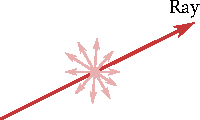
\includegraphics[scale=1]{figures/ch_16/fig_16_1.pdf}
		\caption[]{}
        % \caption[]{Oscillations of natural light occur in the most diverse directions perpendicular to a ray (unpolarized light).}
		\label{fig:16_1}
	\end{center}
	\vspace{-0.8cm}
\end{figure}

Trong ánh sáng tự nhiên, các dao động theo các hướng khác nhau nối tiếp nhau một cách nhanh chóng và không theo bất kỳ trật tự nào.
Ánh sáng mà trong đó hướng của các dao động được đưa vào một trật tự nào đó được gọi là ánh sáng \textbf{phân cực}.
Nếu các dao động của vector ánh sáng chỉ diễn ra trong một mặt phẳng đi qua một tia sáng, ánh sáng đó được gọi là \textbf{sóng phẳng} (hay \textbf{phân cực} \textbf{tuyến tính}) .
Một trật tự khác đó là vector $\vec{E}$ xoay quanh tia sáng trong khi vẫn liên tục thay đổi độ lớn. Kết quả là đầu mút của vector $\vec{E}$ sẽ vẽ ra một đường elip.
Ánh sáng như vậy được gọi là \textbf{ánh sáng phân cực elip}.
Nếu đầu mút của vector $\vec{E}$ vẽ ra một đường tròn, thì ánh sáng đó được gọi là ánh sáng \textbf{phân cực tròn}.

Chúng ta sẽ xem xét ánh sáng tự nhiên trong Chương \ref{chap:17} và Chương \ref{chap:18}.
Vì vậy, chúng ta sẽ không quan tâm đến hướng dao động của vector ánh sáng.
Cách tạo ra ánh sáng phân cực và tính chất của chúng được xem xét trong Chương \ref{chap:19}.

\section{Biểu diễn hàm điều hòa bằng hàm mũ}\label{sec:16_2}

Hãy tính tổng hai số phức $z_1 = x_1 + i y_1$ and $z_2 = x_2 + i y_2$:
\begin{equation}\label{eq:16_11}
    z = z_1 + z_2 = (x_1 + i y_1) + (x_2 + i y_2) = (x_1 + x_2) + i (y_1 + y_2).
\end{equation}

\noindent
Có thể thấy từ \eqn{16_11} phần thực của tổng hai số phức bằng tổng phần thực của các số hạng:
\begin{equation}\label{eq:16_12}
    \Re\bracet{(z_1 + z_2)} = \Re\bracet{z_1} + \Re\bracet{z_2}.
\end{equation}

Giả sử rằng có một số phức là một hàm của một tham số nào đó, ví dụ như thời gian $t$:
\begin{equation*}
    z(t) = x(t) + i y(t).
\end{equation*}

\noindent
Đạo hàm hàm này theo $t$, ta được
\begin{equation*}
    \diff{z}{t} = \diff{x}{t} + i \diff{y}{t}.
\end{equation*}

\noindent
Từ đó cho thấy phần thực của đạo hàm của $z$ theo $t$ bằng đạo hàm phần thực của $z$ theo $t$:
\begin{equation}\label{eq:16_13}
    \Re\bracet{\diff{z}{t}} = \diff{}{t}\Re\bracet{z}.
\end{equation}

Quan hệ tương tự cũng đúng với tích phân của hàm phức.
Ta có,
\begin{equation*}
    \int z(t)\, \deriv{t} = \int x(t)\, \deriv{t} + i \int y(t)\, \deriv{t},
\end{equation*}

\noindent
từ đó có thể thấy rằng phần thực của tích phân của $z(t)$ bằng với tích phân phần thực của $z(t)$:
\begin{equation}\label{eq:16_14}
    \Re\bracet{\int z(t)\, \deriv{t}} = \int \Re\bracket{z(t)\, \deriv{t}}.
\end{equation}

Rõ ràng rằng các mối quan hệ tương tự với các Phương trình. \eqref{eq:16_12}, \eqref{eq:16_13}, and \eqref{eq:16_14} cũng đúng cho phần ảo của các hàm phức.

Từ những điều trên, khi các phép toán cộng, đạo hàm và tích phân cũng như tổ hợp tuyến tính của các phép toán này được thực hiện với các hàm phức, phần thực (ảo) của kết quả sẽ trùng khớp với kết quả thu được khi các phép toán tương tự được thực hiện với các phần thực (ảo) của các hàm đó\footnote{Chú ý rằng quy tắc này không áp dụng cho các toán tử phi tuyến, ví dụ như phép nhân hoặc bình phương các hàm.}.
Sử dụng kí hiệu $\widetilde{L}$ cho một tổ hợp tuyến tính của các phép toán trên, ta có thể viết:
\begin{equation}\label{eq:16_15}
    \Re\bracet{\widetilde{L}(z_1, z_2, \ldots)} = \widetilde{L}(\Re\bracet{z_1}, \Re\bracet{z_2}, \ldots).
\end{equation}

Tính chất mà chúng ta vừa thiết lập của các phép toán tuyến tính cho phép ta sử dụng phương pháp sau trong tính toán: khi thực hiện phép toán tuyến tính với các hàm điều hòa có dạng $A \cos(\omega t - k_x x - k_y y - k_z z + \alpha)$, ta có thể thay thế những hàm này bằng các hàm mũ
\begin{equation}\label{eq:16_16}
    A \exp[i (\omega t - k_x x - k_y y - k_z z + \alpha)] = \hat{A} \exp[i (\omega t - k_x x - k_y y - k_z z)],
\end{equation}

\noindent
trong đó $\hat{A} = A\,e^{i\alpha}$ là một số phức được gọi là \textbf{biên độ phức}.
Với cách biểu diễn như vậy, ta có thể cộng các hàm, đạo hàm chúng theo các biến $t$, $x$, $y$, $z$, và cũng có thể tích phân các hàm theo các biến này.
Để thực hiện phép tính, ta phải lấy phần thực của kết quả thu được.
Lợi ích của phương pháp này là việc tính toán bằng hàm mũ sẽ đơn giản hơn nhiều so với việc tính toán bằng hàm lượng giác.

Khi chuyển sang biểu diễn \eqref{eq:16_16}, thực chất chúng ta đã thêm các số hạng $iA \sin(\omega t - k_x x - k_y y - k_z z + \alpha)$ vào các hàm $A \cos(\omega t - k_x x - k_y y - k_z z + \alpha)$.
Chú ý rằng chúng ta đã sử dụng phương pháp tương tự khi học về dao động cưỡng bức (xem Sec. 7.12 of Tập I).

\section{Sự phản xạ và khúc xạ của một sóng phẳng tại mặt phân cách giữa hai điện môi}\label{sec:16_3}

Giả sử một sóng điện từ phẳng chiếu tới mặt phẳng phân cách giữa hai điện môi đồng nhất và đẳng hướng.
Chất điện môi trong đó sóng tới đang lan truyền được đặc trưng bởi hằng số điện môi $\varepsilon_1$, và điện môi thứ hai được đặc trưng bởi hằng số điện môi $\varepsilon_2$.
Giả sử rằng các hằng số điện môi là thống nhất. Thực nghiệm chỉ ra rằng trong trường hợp này, ngoài một sóng phẳng khúc xạ truyền trong điện môi thứ hai, còn có một sóng phẳng phản xạ truyền trong điện môi thứ nhất được tạo thành.

Ta xác định hướng lan truyền của sóng tới bằng vector sóng $\vec{k}$, của sóng phản xạ bằng vector $\vec{k}'$ và, cuối cùng, của sóng khúc xạ bằng vector $\vec{k}''$.
Ta sẽ xác định xem hướng của $\vec{k}'$ and $\vec{k}''$ liên hệ với hướng của $\vec{k}$ như thế nào.
Để làm điều đó, ta sẽ tận dụng thực tế rằng điều kiện sau đây phải thỏa mãn ở mặt phân cách giữa hai môi trường điện môi:
\begin{equation}\label{eq:16_17}
    E_{1,\tau} = E_{2,\tau}.
\end{equation}

\noindent
Ở đây $E_{1,\tau}$ và $E_{2,\tau}$ lần lượt là các thành phần tiếp tuyến của vector cường độ điện trường ở môi trường thứ nhất và thứ 2.

Trong \sect{2_7}, ta đã chứng minh \eqn{16_17} cho trường tĩnh điện [see \eqn{2_44}].
Tuy nhiên nó cũng có thể dễ dàng được mở rộng cho cả các trường biến thiên theo thời gian.
Theo \eqn{9_5}, lưu số của $\vec{E}$ xác định bởi \eqn{2_42} cho trường biến thiên thì không bằng không, mà bằng tích phân $\int(-\dot{\vec{B}})\ccdot\derivec{S}$ lấy trên toàn bộ diện tích của vòng kín thể hiện trong \fig{2_9}:
\begin{equation*}
    \oint E_l\, \deriv{l} = E_{1,x}a - E_{2,x}a + \average{E_b} 2b = - \int_{S=ab} \dot{\vec{B}} \ccdot \derivec{S}.
\end{equation*}

\noindent
Do $\dot{\vec{B}}$ là hữu hạn, tại giới hạn $b\to 0$ thì tích phân ở vế phải biến mất, và chúng ta tìm được điều kiện \eqref{eq:2_43}, từ đó dẫn đến \eqn{2_44}.

Giả sử vector $\vec{k}$ xác định hướng lan truyền của sóng tới nằm trong mặt phẳng hình vẽ (\fig{16_2}).
Hướng pháp tuyến của mặt phân cách được đặc trưng bởi vector $\hatvec{n}$.
Mặt phẳng chứa các vector $\vec{k}$ và $\hatvec{n}$ được gọi là \textbf{mặt phẳng tới} của sóng.
Chọn giao tuyến giữa mặt phẳng tới và mặt phân cách giữa hai điện môi làm trục $x$.
Hướng trục $y$ vuông góc với mặt phân cách giữa hai điện môi.
Do đó, trục $z$ sẽ hướng vuông góc với mặt phẳng tới, trong khi vector $\hatvec{\tau}$ sẽ hướng theo trục $x$ (xem \fig{16_2}).

\begin{figure}[!htb]
	\begin{center}
		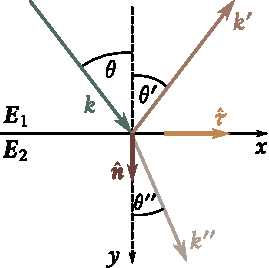
\includegraphics[scale=1]{figures/ch_16/fig_16_2.pdf}
		\caption[]{}
        % \caption[]{Propagation of incident wave ($\vec{k}$), reflecting ($\vec{k}'$) and refracting ($\vec{k}''$)} at an interface. The plane in which the vectors $\vec{k}$ and $\hatvec{n}$ are is called the plane of incidence of the wave.
		\label{fig:16_2}
	\end{center}
	\vspace{-0.8cm}
\end{figure}

Khi xét đến sự đối xứng, rõ ràng rằng các vector $\vec{k}'$ và $\vec{k}''$ chỉ có thể nằm trong mặt phẳng tới (các môi trường là đồng nhất và đẳng hướng).
Thật vậy, giả sử vector $\vec{k}'$ bị lệch khỏi mặt phẳng tới ``về phía chúng ta''.
Tuy nhiên, không có căn cứ nào để ưu tiên sự lệch như vậy so với sự lệch tương đương ``ra xa chúng ta''.
Do đó, hướng khả dĩ duy nhất của vector $\vec{k}'$ là nằm trong mặt phẳng tới. Lập luận tương tự cũng đúng cho vector $\vec{k}''$.

Bây giờ tách ra từ tia sáng tự nhiên chiếu tới mặt phân cách một thành phần phân cực phẳng có hướng dao động của vector $\vec{E}$ lập một góc bất kì với mặt phẳng tới.
Sự dao động của vector $\vec{E}$ trong mặt phẳng mà sóng điện từ lan truyền theo hướng vector $\vec{k}$ được mô tả bởi hàm\footnote{Chính xác hơn là phần thực của hàm, nhưng ta sẽ chỉ nói đơn giản là hàm cho ngắn gọn.}
\begin{equation*}
    \vec{E} = \ab{\vec{E}}{m} \exp[i (\omega t - \vecdot{k}{r})] = \ab{\vec{E}}{m} \exp[i (\omega t - k_x x - k_y y)]
\end{equation*}

\noindent
(với việc chọn các trục như ta đã làm, hình chiếu của vector $\vec{k}$ lên phương $z$ là bằng không, do đó số hạng $-k_zz$ bị triệt tiêu ở số mũ).
Ta cũng đã chọn mốc thời gian sao cho pha ban đầu của sóng tương ứng bằng không.

Cường độ của trường trong sóng phản xạ và khúc xạ cũng được mô tả bằng các biểu thức tương tự
\begin{align*}
    \vec{E}' &= \ab{\vec{E}}{m}' \exp[i (\omega t - k_x' x - k_y' y + \alpha')]\\
    \vec{E}'' &= \ab{\vec{E}}{m}'' \exp[i (\omega t - k_x'' x - k_y'' y + \alpha'')],
\end{align*}

\noindent
với $\alpha'$ và $\alpha''$ là pha ban đầu của sóng tương ứng.

Trường tổng hợp trong môi trường thứ nhất là
\begin{align}
    \vec{E}_1 = \vec{E} + \vec{E}' = \ab{\vec{E}}{m} \exp[i (\omega t &- k_x x - k_y y + \alpha)] \nonumber\\
    &+ \ab{\vec{E}}{m}' \exp[i (\omega t - k_x' x - k_y' y + \alpha')].\label{eq:16_18}
\end{align}

\noindent
Trong môi trường thứ hai
\begin{equation}\label{eq:16_19}
    \vec{E}_2 = \vec{E}'' = \ab{\vec{E}}{m}'' \exp[i (\omega t - k_x'' x - k_y'' y + \alpha'')].
\end{equation}

\noindent
Theo \eqn{16_17}, thành phần tiếp tuyến của \eqns{16_18}{16_19} phải giữ nguyên ở mặt phân cách,tức là khi $y = 0$.
Từ đó dẫn đến biểu thức
\begin{align}
    \ab{E}{m,$\tau$} \exp[i(\omega t - k_xx)] + \ab{E}{m,$\tau$}' &\exp[i(\omega' t - k_xx' + \alpha')] \nonumber\\
    &= \ab{E}{m,$\tau$}'' \exp[i(\omega'' t - k_xx + \alpha'')].\label{eq:16_20}
\end{align}

Để điều kiện \eqref{eq:16_20} thỏa mãn tại $t$ bất kì, các tần số đều phải bằng nhau:
\begin{equation}\label{eq:16_21}
    \omega = \omega' = \omega''.
\end{equation}

\noindent
Để tự thuyết phục mình rằng điều này là đúng, hãy viết \eqn{16_20} dưới dạng
\begin{equation*}
    a \exp(i\omega t) + b \exp(i\omega' t) = c\exp(i\omega'' t),
\end{equation*}

\noindent
với các hệ số $a$, $b$, và $c$ là độc lập với $t$.
Phương trình ta vừa viết tương đương với hai phương trình sau:
\begin{align*}
    a \cos(\omega t) + b \cos(\omega' t) &= c \cos(\omega'' t)\\
    a \sin(\omega t) + b \sin(\omega' t) &= c \sin(\omega'' t).
\end{align*}

\noindent
Tổng của hai hàm điều hòa cũng là một hàm điều hào chỉ khi các hàm được cộng có cùng tần số.
Hàm điều hòa mới nhận được cũng sẽ có cùng tần số với các hàm ban đầu.
Từ đó dẫn đến \eqn{16_21}.
Vì vậy, ta đi đến kết luận rằng tần số của sóng phản xạ và khúc xạ trùng với tần số của sóng tới.

Để điều kiện \eqref{eq:16_20} thỏa mãn với $x$ bất kì, hình chiếu của các vector sóng lên trục $x$ phải bằng nhau:
\begin{equation}\label{eq:16_22}
    k_x = k_x' = k_x''.
\end{equation}

\noindent
Các góc $\theta$, $\theta'$, và $\theta''$ thể hiện \fig{16_2} được gọi là \textbf{góc tới}, the \textbf{góc phản xạ}, và \textbf{góc khúc xạ}.
Dựa vào hình vẽ ta có $k_x = k\sin\theta$, $k_x' = k'\sin\theta'$, $k_x'' =
= k''\sin\theta''$.
\eqref{eq:16_22} do đó có thể viết dưới dạng
\begin{equation*}
    k \sin\theta = k' \sin\theta' = k'' \sin\theta''.
\end{equation*}

\noindent
Các vector $\vec{k}$ và $\vec{k}'$ có cùng độ lớn và bằng $\omega/v_1$; độ lớn của vector $\vec{k}''$ bằng $w/v_2$.
Do đó,
\begin{equation*}
    \frac{\omega}{v_1} \sin\theta = \frac{\omega}{v_1} \sin\theta' = \frac{\omega}{v_2} \sin\theta''.
\end{equation*}

\noindent
Vì vậy dẫn đến
\begin{align}
    \theta' &= \theta, \label{eq:16_23}\\
    \frac{\sin\theta}{\sin\theta''} &= \frac{v_1}{v_2} = n_{12}. \label{eq:16_24}
\end{align}

Các quan hệ ta vừa nhận được thỏa mãn với mọi thành phần phân cực phẳng bất kì của một tia sáng tự nhiên.
Do đó, chúng cũng đúng cả cho một tia sáng tự nhiên.

\eqref{eq:16_23} biểu diễn \textbf{định luật phản xạ ánh sáng}, theo đó \textit{tia phản xạ nằm trong mặt phẳng chứa tia tới và pháp tuyến tại điểm tới; góc phản xạ bằng góc tới}.

\eqref{eq:16_24} biểu diễn \textbf{định luật khúc xạ ánh sáng}, theo đó \textit{tia phản xạ nằm trong mặt phẳng chứa tia tới và pháp tuyến tại điểm tới; tỉ số giữa sin góc tới và sin góc khúc xạ là hằng số với mỗi chất cho trước}.

Đại lượng $n_{12}$ trong \eqn{16_24} gọi là \textbf{chiết suất tỉ đối} của chất thứ hai so với chất thứ nhất.
Hãy viết đại lượng này dưới dạng
\begin{equation}\label{eq:16_25}
    n_{12} = \frac{v_1}{v_2} = \frac{c}{v_2} \frac{v_1}{c} = \frac{c/v_2}{c/v_1} = \frac{n_2}{n_1}.
\end{equation}

\noindent
Từ đó, chiết suất tỉ đối của hai chất bằng tỉ số chiết suất tuyệt đối của chúng.

Thay $n_2/n_1$ cho $n_{12}$ trong \eqn{16_24}, ta có thể viết định luật khúc xạ dưới dạng
\begin{equation}\label{eq:16_26}
    n_1 \sin\theta = n_2 \sin\theta''.
\end{equation}

\noindent
Xem xét kĩ hơn phương trình này cho thấy khi ánh sáng truyền từ một môi trường chiết quang hơn sang một môi trường kém chiết quang hơn, các tia sáng sẽ lệch ra xa pháp tuyến về phía mặt phân cách giữa các môi trường.
Khi góc tới $\theta$ tăng lên thì góc khúc xạ $\theta''$ cũng tăng, nhưng tăng nhanh hơn; và khi góc $\theta$ đạt giá trị
\begin{equation}\label{eq:16_27}
    \ab{\theta}{cr} = \arcsin n_{12},
\end{equation}

\noindent
thì góc $\theta''$ đạt $\pi/2$.
Góc xác định bởi \eqn{16_27} được gọi là \textbf{góc tới hạn}.

Năng lượng của tia tới được phân bổ cho tia phản xạ và tia khúc xạ.
Khi góc tới tăng lên, cường độ của sóng phản xạ tăng lên, trong khi cường độ của sóng khúc xạ giảm dần rồi hoàn toàn bị triệt tiêu khi góc tới đạt giá trị tới hạn.
Khi góc tới có giá trị nằm trong khoảng từ $\ab{\theta}{cr}$ đến $\pi/2$, sóng ánh sáng chỉ đi vào môi trường thứ hai một đoạn có độ dài cỡ bước sóng $\lambda$ rồi trở lại môi trường thứ nhất.
Hiện tượng này được gọi là \textbf{sự phản xạ toàn phần}.

Bây giờ ta sẽ tìm mối quan hệ giữa biên độ và pha của sóng tới, sóng phản xạ và sóng khúc xạ.
Để đơn giản, chúng ta sẽ chỉ xét trường hợp sóng tới theo phương pháp tuyến của mặt phân cách giữa hai điện môi (lưu ý rằng các điện môi được coi là đồng nhất và đẳng hướng).
Giả sử rằng dao động của vector $\vec{E}$ trong sóng tới diễn ra theo hướng trục $x$.
Việc xem xét sự đối xứng chỉ ra rằng sự dao động của các vector $\vec{E}'$ và $\vec{E}''$ cũng diễn ra theo trục $x$.
Trong trường hợp này, vector đơn vị $\hatvec{\tau}$ trùng với vector đơn vị $\vecuni{x}$.
Do đó, điều kiện liên tục của thành phần cường độ điện trường theo phương tiếp tuyến có dạng
\begin{equation}\label{eq:16_28}
    E_x + E_x' = E_x''.
\end{equation}

Biểu thức \eqref{eq:16_8} cho biên độ của $E$ và $H$ vẫn đúng cho các giá trị tức thời của các vector này: $H \propto nE$.
Do đó, giá trị tức thời của mật độ năng thông tỉ lệ với $nE^2$.
Từ đó, định luật bảo toàn năng lượng dẫn đến phương trình
\begin{equation}\label{eq:16_29}
    n_1 E_x^2 = n_1 E_x'^2 + n_2 E_x''^2.
\end{equation}

\noindent
Chú ý rằng các đại lượng $E_x$, $E_x'$ và $E_x''$ trong \eqns{16_28}{16_29} là các giá trị tức thời của các hình chiếu.

Thay $E_x'$ trong \eqn{16_29} bằng $E_x''-E_x$  [xem \eqn{16_28}], dễ thấy rằng
\begin{equation}\label{eq:16_30}
    E_x'' = \parenthesis{\frac{2 n_1}{(n_1 + n_2)}} E_x.
\end{equation}

\noindent
Thay giá trị này của $E_x''$ vào \eqn{16_28}, ta tìm được
\begin{equation}\label{eq:16_31}
    E_x' = \parenthesis{\frac{n_1 - n_2}{n_1 + n_2}} E_x.
\end{equation}

Tại một thời điểm bất kì, \eqn{16_30} cho thấy hình chiếu của các vector $\vec{E}$ và $\vec{E}''$ cùng dấu.
Do đó, ta kết luận rằng các dao động của sóng tới và sóng truyền sang môi trường thứ hai cùng pha nhau tại mặt phân cách---khi sóng truyền qua mặt phân cách thì không có sự thay đổi về pha.

Có thể thấy từ \eqn{16_31} rằng khi $n_2 < n_1$, dấu của $E_x'$ trùng với dấu của $E_x$.
Điều này có nghĩa là các dao động của sóng tới và sóng phản xạ cùng pha nhau tại mặt phân cách---pha của sóng không thay đổi khi phản xạ.
Nếu $n_2 > n_1$, thì dấu của $E_x'$ trái với dấu của $E_x$, các dao động của sóng tới và sóng phản xạ ngược pha nhau tại mặt phân cách---pha của sóng tăng một lượng $\pi$ khi phản xạ.
Kết quả này cũng đúng với một sóng chiếu xiên tới mặt phân cách giữa hai môi trường trong suốt.

Vì vậy, khi sóng ánh sáng từ môi trường kém chiết quang hơn đến phản xạ trên mặt phân cách với môi trường chiết quang hơn (tức là khi $n_1 < n_2$), pha dao động của sóng ánh sáng sẽ thay đổi một lượng $\pi$.
Sự thay đổi pha như vậy không xảy ra khi phản xạ trên mặt phân cách với môi trường kém chiết quang hơn (khi $n_1 > n_2$).

Các phương trình \eqref{eq:16_30} và \eqref{eq:16_31} được viết cho các giá trị tức thời của hình chiếu vector ánh sáng.
Các quan hệ tương tự cũng đúng với biên độ của các vector ánh sáng:
\begin{equation}\label{eq:16_32}
    \ab{E}{m}'' = \parenthesis{\frac{2 n_1}{(n_1 + n_2)}} \ab{E}{m},\quad \ab{E}{m}' = \absolute{\frac{n_1 - n_2}{n_1 + n_2}} \ab{E}{m}.
\end{equation}

\noindent
Các quan hệ này cho phép tìm hệ số phản xạ $\rho$ và hệ số truyền $\tau$ của một sóng ánh sáng (chiếu tới mặt phân cách giữa hai môi trường trong suốt theo phương pháp tuyến).
Thực vậy, từ định nghĩa
\begin{equation*}
    \rho = \frac{I'}{I} = \frac{n_1 \ab{E}{m}'^2}{n_1 \ab{E}{m}^2},
\end{equation*}

\noindent
với $I'$ là cường độ của sóng phản xạ, và $I$ là cường độ của sóng tới.
Áp dụng tỉ số $\ab{E}{m}'/\ab{E}{m}$ nhận được từ \eqn{16_32} vào phương trình này, ta thu được công thức
\begin{equation}\label{eq:16_33}
    \rho = \parenthesis{\frac{n_{12} - 1}{n_{12} + 1}}^2.
\end{equation}

\noindent
Ở đây, $n_{12} = n_2/n_1$ là chiết suất tương đối của môi trường thứ hai so với môi trường thứ nhất.

Ta cũng thu được biểu thức sau cho hệ số truyền:
\begin{equation}\label{eq:16_34}
    \tau = \frac{I''}{I} = \frac{n_2 \ab{E}{m}''^2}{n_1 \ab{E}{m}^2} = n_{12} \parenthesis{\frac{2}{n_{12} + 1}}^2.
\end{equation}

Chú ý rằng việc thay thế $n_{12}$ trong \eqn{16_33} bằng nghịch đảo của nó $n_{21} = 1/n_{12}$ không làm thay đổi giá trị của $\rho$.
Do đó, hệ số phản xạ của mặt phân cách giữa hai môi trường cho trước có cùng giá trị đối với cả hai hướng truyền của ánh sáng.

Chiết suất chủa thủy tinh gần bằng $1.5$. Thay $n_{12} = 1.5$ vào \eqn{16_33}, ta được $\rho = 0.04$.
Tức là, mỗi bề mặt thủy tinh phản xạ khoảng bốn phần trăm quang năng chiếu tới nó (theo phương gần với phương pháp tuyến).

\section{Quang thông}\label{sec:16_4}

Sóng ánh sáng trong thực tế là sự chồng chập các sóng có bước sóng giới hạn trong một khoảng $\Delta{\lambda}$.
Khoảng này cũng tồn tại ngay cả với ánh sáng đơn sắc (chỉ có một màu).
Trong ánh sáng trắng, $\Delta{\lambda}$ phủ toàn bộ dải sóng điện từ mà mắt người cảm nhận được, tức là nằm trong khoảng từ \SI{0.40}{\micro\metre} đến \SI{0.76}{\micro\metre}.

Sự phân bố năng thông theo bước sóng đước đặc trưng bởi hàm phân bố
\begin{equation}\label{eq:16_35}
    \varphi(\lambda) = \diff{\ab{\Phi}{en}}{\lambda},
\end{equation}

\noindent
với $\deriv{\ab{\Phi}{en}}$ là năng thông của các sóng có bước sóng từ $\lambda$ đến $\lambda+\Delta{\lambda}$.
Nếu biết được dạng của hàm \eqref{eq:16_35}, ta có thể tính năng thông được truyền bởi các sóng có bước sóng nằm trong khoảng từ $\lambda_1$ đến $\lambda_2$:
\begin{equation}\label{eq:16_36}
    \ab{\Phi}{en} = \int_{\lambda_1}^{\lambda_2} \varphi(\lambda)\, \deriv{\lambda}.
\end{equation}

\noindent
Tác dụng của ánh sáng lên mắt (sự cảm nhận ánh sáng) phụ thuộc khá nhiều vào bước sóng.
Điều này cũng dễ hiểu vì các sóng điện từ với $\lambda$ nhỏ hơn \SI{0.40}{\micro\metre} và lớn hơn \SI{0.76}{\micro\metre} đều không thể được cảm nhận bởi mắt người.
Độ nhạy của mắt người trung bình với bức xạ của các bước sóng khác nhau có thể được mô tả trực quan bằng một \textbf{đường độ nhạy quang phổ tương đối} (\fig{16_3}).
Trục nằm ngang biểu diễn bước sóng $\lambda$, còn trục thẳng đứng biểu diễn độ nhạy quang phổ tương đối $V(\lambda)$.
Mắt nhạy nhất với bức xạ của bước sóng \SI{0.555}{\micro\metre}\footnote{Điều thú vị là bước sóng này cũng là bước sóng có cường độ lớn nhất trong bức xạ mặt trời.} (phần màu xanh của phổ).
Hàm $V(\lambda)$ ở bước sóng này được chọn là một đơn vị.
Cường độ sáng ước tính trực quan cho các bước sóng khác thấp hơn, mặc dù năng thông là như nhau.
Theo đó, $V(\lambda)$ cho các bước sóng này cũng nhỏ hơn một.
Các giá trị của hàm $V(\lambda)$ tỷ lệ nghịch với các giá trị của năng thông tạo ra cảm giác thị giác giống hệt nhau về cường độ:
\begin{equation*}
    \frac{V(\lambda_1)}{V(\lambda_2)} = \frac{(\deriv{\ab{\Phi}{en}})_2}{(\deriv{\ab{\Phi}{en}})_1}.
\end{equation*}

\begin{figure}[!htb]
	\begin{center}
		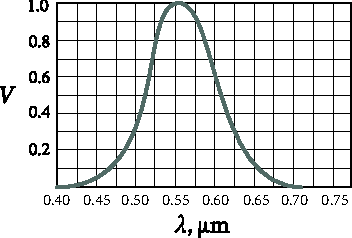
\includegraphics[scale=1]{figures/ch_16/fig_16_3.pdf}
		\caption[]{}
        % \caption[]{Curve of relative spectral sensitivity: sensitivity of an average normal human eye to radiation of various wavelengths.}
		\label{fig:16_3}
	\end{center}
	\vspace{-0.8cm}
\end{figure}

\noindent
Ví dụ, $V(\lambda) = 0.5$ cho biết rằng để có được cảm nhận thị giác ở cùng cường độ, ánh sáng ở bước sóng trên phải có một độ năng thông gấp đôi so với ánh sáng ở bước sóng $V(\lambda)=1$.
Ở ngoài vùng ánh sáng nhìn thấy, hàm $V(\lambda)$ bằng không.

Đại lượng $\Phi$ được gọi là \textbf{quang thông}, đặc trưng cho cường độ sáng về khả năng tạo ra cảm nhận thị giác.
Trong khoảng $\deriv{\lambda}$, quang thông được xác định bằng tích của năng thông với giá trị tương ứng của hàm $V(\lambda)$:
\begin{equation}\label{eq:16_37}
    \deriv{\Phi} = V(\lambda)\, \deriv{\ab{\Phi}{en}}.
\end{equation}

\noindent
Biểu diễn năng thông qua hàm phân bố năng lượng theo bước sóng [xem \eqn{16_35}], ta được
\begin{equation}\label{eq:16_38}
    \deriv{\Phi} = V(\lambda) \varphi(\lambda)\, \deriv{\lambda}.
\end{equation}

\noindent
Quang thông tổng cộng là
\begin{equation}\label{eq:16_39}
    \Phi = \int_0^{\infty} V(\lambda) \varphi(\lambda)\, \deriv{\lambda}.
\end{equation}

Hàm $V(\lambda)$ là một đại lượng không thứ nguyên.
Do đó, thứ nguyên của quang thông trùng với thứ nguyên của năng thông.
Điều này cho phép định nghĩa quang thông như là năng thông được đánh giá dựa trên cảm nhận thị giác.

\section{Các đại lượng và đơn vị trắc quang}\label{sec:16_5}

Trắc quang là một nhánh của quang học liên quan đến việc đo đạc quang thông và các đại lượng liên quan.

\textbf{Cường độ sáng}
Một nguồn sáng mà kích thước có thể bỏ qua so với khoảng cách từ điểm quan sát tới nguồn sáng đó được gọi là một \textbf{nguồn sáng điểm}.
Trong môi trường đồng nhất và đẳng hướng, sóng phát ra từ một nguồn sáng điểm là sóng cầu.
Nguồn sáng điểm được đặc trưng bởi cường độ sáng $I$, được định nghĩa là quang thông phát ra trên một đơn vị góc khối:
\begin{equation}\label{eq:16_40}
    I = \diff{\Phi}{\Omega}
\end{equation}

\noindent
$\deriv{\Phi}$ là năng thông phát ra bởi nguồn trong phạm vi góc khối $\deriv{\Omega}$).

Trong trường hợp tổng quát, cường độ sáng có phụ thuộc vào hướng: $I=I(\theta,\varphi)$ (ở đây $\theta$ và $\varphi$ là góc cực và góc phương vị trong hệ tọa độ cầu).
Nếu $I$ không phụ thuộc vào hướng, thì nguồn sáng điểm được gọi là \textbf{đẳng hướng}.
Với nguồn đẳng hướng
\begin{equation}\label{eq:16_41}
    I = \frac{\Phi}{4\pi},
\end{equation}

\noindent
với $\Phi$ là tổng quang thông phát ra bởi nguồn theo mọi hướng.

Khi làm việc với một nguồn sáng có kích thước, ta có thể nói về cường độ sáng của một phần tử diện tích trên bề mặt nguồn sáng $\deriv{S}$.
Now by $\deriv{\Phi}$ in \eqn{16_40} we must understand the luminous flux emitted by the surface
element $\deriv{S}$ within the limits of the solid angle $\deriv{\Omega}$.

Đơn vị của cường độ sáng--- candela (\si{\candela}) là một đơn vị cơ bản trong hệ đơn vị SI.
Nó được định nghĩa là cường độ sáng theo phương vuông của bề mặt có diện tích $1/600000$ mét vuông của một bộ tản nhiệt hoàn chỉnh ở nhiệt độ đông đặc của bạch kim dưới áp suất $101325$ pascal.
Ở đây một bộ tản nhiệt hoàn chỉnh nghĩa là một thiết bị có các tính chất của một vật đen (Xem Tâp III).

\textbf{Quang thông.}
Đơn vị của quang thông là lumen (\si{\lumen}).
Nó bằng quang thông phát ra bởi một nguồn sáng đẳng hướng với cường độ sáng $1$ candela trong phạm vi góc khối một steradian:
\begin{equation}\label{eq:16_42}
    \SI{1}{\lumen} = \SI{1}{\candela} \cdot \SI{1}{\steradian}.
\end{equation}

Thực nghiệm đã thiết lập rằng một năng thông có giá trị \SI{0.0016}{\watt} tương ứng với một quang thông có giá trị \SI{1}{\lumen} của bức xạ có bước sóng $\lambda = \SI{0.555}{\micro\metre}$.
Năng thông
\begin{equation}\label{eq:16_43}
    \ab{\Phi}{en} = \frac{0.0016}{V(\lambda)} \si{\watt},
\end{equation}

\noindent
tương ứng với quang thông \SI{1}{\lumen} của bức xạ của các bước sóng khác.

\textbf{Độ rọi.}
Độ sáng của một bề mặt do tác dụng của ánh sáng chiếu đến được đặc trưng bởi đại lượng
\begin{equation}\label{eq:16_44}
    E = \diff{\ab{\Phi}{inc}}{S},
\end{equation}

\noindent
được gọi là \textbf{độ rọi} ($\deriv{\ab{\Phi}{inc}}$ là quang thông chiếu tới phần tử bề mặt $\deriv{S}$).

Đơn vị của độ rọi là (\si{\lux}), bằng độ rọi do quang thông một \SI{1}{\lumen} phân bố đều trên một bề mặt có diện tích \SI{1}{\metre\squared}:
\begin{equation}\label{eq:16_45}
    \SI{1}{\lux} = \SI{1}{\lumen} : \SI{1}{\metre\squared}.
\end{equation}

Độ rọi $E$ gây ra bởi một nguồn sáng điểm có thể được biếu diễn thông qua cường độ sáng $I$, khoảng cách $r$ từ bề mặt tới nguồn, và góc $\alpha$ giữa pháp tuyến của bề mặt $\hatvec{n}$ với hướng tới nguồn.
quang thông chiếu tới diện tích $\deriv{S}$ (\fig{16_4}) là $\deriv{\ab{\Phi}{inc}}=I\, \deriv{\Omega}$ và nó bị giới hạn trong góc khối $\deriv{\Omega}$ đối diện diện tích $\deriv{S}$.
Góc $\deriv{\Omega}$ là $\deriv{S}\cos\alpha/r^2$.
Do đó, $\deriv{\ab{\Phi}{inc}}=I\,\deriv{S} \cos\alpha/r^2$.
Chia quang thông này cho $\deriv{S}$, ta được
\begin{equation}\label{eq:16_46}
    E = \frac{I \cos\alpha}{r^2}.
\end{equation}

\begin{figure}[!htb]
	\begin{center}
		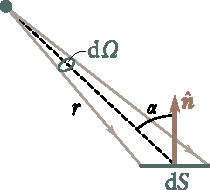
\includegraphics[scale=1]{figures/ch_16/fig_16_4.pdf}
		\caption[]{}
        % \caption[]{Incident flux $\deriv{\ab{\Phi}{inc}}$ on area $\deriv{S}$ confined by the solid angle $\deriv{\Omega}$.}
		\label{fig:16_4}
	\end{center}
	\vspace{-0.8cm}
\end{figure}

\textbf{Độ trưng.}
Một nguồn sáng có kích thước có thể được đặc trưng bởi độ trưng $M$ của từng phần, với ý nghĩa là quang thông phát ra từ một đơn vị diện tích theo mọi hướng (trong giới hạn của góc $\theta$ là từ $0$ đến $\pi/2$, với $\theta$ là góc tạo bởi hướng cho trước với pháp tuyến hướng ra ngoài của bề mặt):
\begin{equation}\label{eq:16_47}
    M = \diff{\ab{\Phi}{em}}{S}
\end{equation}

\noindent
($\deriv{\ab{\Phi}{em}}$ là thông lượng phát ra theo mọi hướng của phần tử bề mặt $\deriv{S}$ của nguồn).

Độ trưng có thể hiểu là kết quả của sự phản xạ ánh sáng chiếu tới một bề mặt.
Ở đây, ta phải hiểu $\deriv{\ab{\Phi}{em}}$ trong \eqn{16_47} là quang thông phản xạ bởi phần tử bề mặt $\deriv{S}$ theo mọi hướng.

Đơn vị của độ trưng là lumen trên mét vuông (\si{\lumen\per\metre\squared}).

\textbf{Độ chói.}
Độ trưng đặc trưng cho sự bức xạ (hay phản xạ) của ánh sáng từ một nguồn theo mọi hướng.
Còn sự bức xạ (hay phản xạ) của ánh sáng theo một hướng cho trước được đặc trưng bởi độ chói $L$.
Hướng ở đây được xác định bởi góc cực $\theta$ (đo được từ pháp tuyến hướng ra ngoài $\hatvec{n}$ của bề mặt phát ra bức xạ $\Delta{S}$) và góc phương vị $\varphi$.
Đọ chới được định nghĩa là tỉ số giữa cường độ sáng của một phần tử diện tích $\Delta{S}$ theo một hướng xác định với hình chiếu của diện tích $\Delta{A}$ lên mặt phẳng vuông góc với hướng đã chọn.

Xét một phần tử góc khối $\deriv{\Omega}$ đối diện với diện tích phát sáng $\deriv{S}$ và được có hướng $(\theta, \varphi)$ (\fig{16_5}).
Cường độ sáng của diện tích $\Delta{S}$ theo một hướng xác định, theo \eqn{16_40}, là $I = \diffin{\Phi}{\Omega}$, với $\deriv{\Phi}$ là quang thông lan truyền trong phạm vi góc khối $\deriv{\Omega}$.
Hình chiếu của $\Delta{S}$ lên mặt phẳng vuông góc với $(\theta, \varphi)$ (trong \fig{16_5} mặt phẳng này được mô tả bằng đường nét đứt) là $\Delta{S}\cos\theta$.
Do đó, độ chói là
\begin{equation}\label{eq:16_48}
    L = \frac{\deriv{\Phi}}{\deriv{\Omega} \Delta{S} \cos\theta}.
\end{equation}

\begin{figure}[!htb]
	\begin{center}
		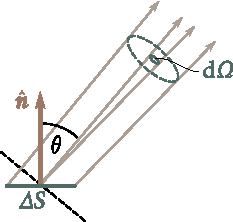
\includegraphics[scale=1]{figures/ch_16/fig_16_5.pdf}
		\caption[]{}
        % \caption[]{Elementary solid angle $\deriv{\Omega}$ subtended by the luminous area $\Delta{S}$ and oriented in the direction $(\theta,\varphi)$.}
		\label{fig:16_5}
	\end{center}
	\vspace{-0.8cm}
\end{figure}

Trong trường hợp tổng quát, độ chói thay đổi theo hướng được chọn : $L=L(\theta,\varphi)$.
Cũng giống như độ trưng, độ chói có thể được dùng để đặc trưng cho một bề mặt phản xạ ánh sáng chiếu đến nó.

Theo \eqn{16_48}, quang thông phát ra bởi diện tích $\Delta{S}$ trong phạm vi góc khối $\deriv{\Omega}$ theo hướng được xác định bởi $\theta$ và $\varphi$ là
\begin{equation}\label{eq:16_49}
    \deriv{\Phi} = L(\theta,\varphi)\, \deriv{\Omega} \Delta{S} \cos\theta.
\end{equation}

Một nguồn sáng có độ chói theo mọi hướng là như nhau ($L = \text{constant}$) được gọi là một \textbf{nguồn sáng Lambert} (tuân theo định luật Lambert) hay một nguồn sáng dạng cosin (quang thông phát ra bởi một phần tử bề mặt của nguồn sáng tỉ lệ với $\cos\theta$).
Chỉ có duy nhất các vật đen là thỏa mãn chặt chẽ định luật Lambert.

Độ trưng $M$ và độ chói $L$ của một nguồn sáng Lambert được liên hệ bởi một biểu thức đơn giản.
Để tìm biểu thức đó, ta thay $\deriv{\Omega}= \sin\theta\,\deriv{\theta}\,\deriv{\varphi}$ vào \eqn{16_49} rồi tích phân biểu thức nhận được theo $\varphi$ trong khoảng từ $0$ đến $2\pi$ và theo $\theta$ trong khoảng từ $0$ đến $\pi/2$, chú ý rằng $L=\text{hằng số}$.
Từ đó, ta sẽ tìm được quang năng tổng cộng phát ra theo mọi hướng bởi phần tử diện tích $\Delta{S}$ của một nguồn sáng Lambert:
\begin{equation*}
    \Delta{\ab{\Phi}{em}} = L \Delta{S} \int_0^{2\pi} \deriv{\varphi} \int_0^{\pi/2} \sin\theta \cos\theta\, \deriv{\theta} = \pi L \Delta{S}.
\end{equation*}

\noindent
Ta sẽ thu được độ trưng bằng cách chia cho $\Delta{S}$.
Do đó, với một nguồn sáng Lambert, ta có
\begin{equation}\label{eq:16_50}
    M = \pi L.
\end{equation}

Đơn vị của độ chói là candela trên mét vuông (\si{\candela\per\metre\squared}).
Một mặt phẳng sáng đều có độ chói \SI{1}{\candela\per\metre\squared} theo phương pháp tuyến với mặt phẳng đó nếu theo hướng này cường độ sáng của một phần diện tích một mét vuông là một candela.

\section{Quang hình học}\label{sec:16_6}
\vspace{-12pt}
Độ dài bước sóng ánh sáng cảm nhận được bởi mắt người là rất nhỏ (cỡ \SI{e-7}{\metre}).
Vì lý do này, có thể xem xét sự lan truyền của ánh sáng khả kiến trong phép gần đúng bậc nhất mà không cần quan tâm đến bản chất sóng của nó và giả sử rằng ánh sáng truyền theo các đường gọi là các \textbf{tia sáng}.
Trong trường hợp giới hạn $\lambda\to 0$, các định luật của quang học có thể được diễn tả bằng ngôn ngữ hình học.

Vì vậy, lĩnh vực quang học mà ở đó ta bỏ qua kích thước của bước sóng được gọi là \textbf{Quang hình học} hay \textbf{quang học về tia sáng}.

Quang hình học dựa trên bốn định luật: (1) định luật truyền thẳng của ánh sáng (2) định luật về tính độc lập của tia sáng; (3) định luật phản xạ ánh sáng; và (4) định luật khúc xạ ánh sáng.

\textbf{Định luật truyền thẳng} phát biểu rằng \textit{trong một môi trường đồng nhất, ánh sáng truyền đi theo đường thẳng}.
Định luật này chỉ là gần đúng---khi ánh sáng có thể bị lệch hướng khi truyền qua một lỗ rất nhỏ, kích thước của lỗ càng nhỏ thì sự lệch hướng quan sát được càng lớn.

\textbf{Định luật về tính độc lập của tia sáng} phát biểu rằng \textit{các tia sáng không làm ảnh hưởng đến các tia sáng khác khi cúng giao nhau}.
Sự giao nhau của tia sáng không cản trở việc chúng truyền đi độc lập với nhau. Định luật này chỉ đúng khi cường độ áng sáng không quá lớn.
Ở cường độ của các tia laser, sự độc lập của các tia sáng không còn đúng nữa.

Các định luật phản xạ và khúc xạ ánh sáng đã được rút ra trong \sect{16_3} [xem \eqns{16_23}{16_24} và diễn giải đi kèm].

Quang hình học cũng có thể được xây dựng dựa trên nguyên lý của nhà toán học người Pháp Pierre de Fermat (1601-1665).
Nó làm cơ sở cho các định luật truyền thẳng, phản xạ và khúc xạ ánh sáng. Theo công thức của chính Fermat, nguyên lý này phát biểu rằng \textit{mọi tia sáng truyền từ điểm này đến điểm khác theo con đường cần thời gian cực tiểu}.

Ánh sáng cần thời gian $\deriv{t} = \deriv{s}/v$ để đi hết quãng đường $\deriv{s}$ (\fig{16_6}), với $v$ là vận tốc ánh sáng tại một điểm cho trước trong môi trường.
Thay $v$ bằng $c/n$ [xem \eqn{16_2}], ta tìm được $\deriv{t}=(1/c)n\,\deriv{s}$.
Do đó, thời gian $\tau$ ánh sáng cần để đi từ điểm $1$ đến điểm $2$ là
\begin{equation}\label{eq:16_51}
    \tau = \frac{1}{c} \int_1^2 n\, \deriv{s}.
\end{equation}

% \begin{figure}[t]
% 	\begin{center}
% 		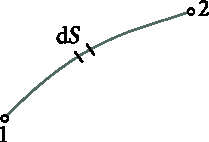
\includegraphics[scale=1]{figures/ch_16/fig_16_6.pdf}
% 		\caption[]{}
%         % \caption[]{Light ray travelling from point 1 to point 2, taking a time $\deriv{t}$ to cover a distance $\deriv{s}$ at speed $v$.}
% 		\label{fig:16_6}
% 	\end{center}
% 	\vspace{-0.8cm}
% \end{figure}
\begin{figure}[!htb]
	\begin{minipage}[t]{0.48\linewidth}
		\begin{center}
			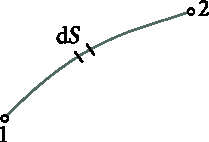
\includegraphics[scale=1]{figures/ch_16/fig_16_6.pdf}
			\caption[]{}
            % \caption[]{Light ray travelling from point 1 to point 2, taking a time $\deriv{t}$ to cover a distance $\deriv{s}$ at speed $v$.}
			\label{fig:16_6}
		\end{center}
	\end{minipage}
	\hfill{ }%space{-0.05cm}
	\begin{minipage}[t]{0.48\linewidth}
		\begin{center}
			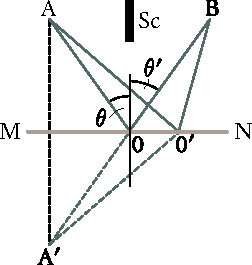
\includegraphics[scale=1]{figures/ch_16/fig_16_7.pdf}
            \caption[]{}
			% \caption[]{Reflection and refraction of light using Fermat's principle.}
			\label{fig:16_7}
		\end{center}
	\end{minipage}
\vspace{-0.4cm}
\end{figure}

Đại lượng
\begin{equation}\label{eq:16_52}
    L = \int_1^2 n\, \deriv{s}
\end{equation}

\noindent
có thứ nguyên độ dài được gọi là \textbf{quang trình}.
Trong một môi trường đồng nhất, quang trình bằng tích của quãng đường hình học $s$ với chiết suất $n$ của môi trường:
\begin{equation}\label{eq:16_53}
    L = ns.
\end{equation}

Theo \eqns{16_51}{16_52}, ta có
\begin{equation}\label{eq:16_54}
    \tau = \frac{L}{c}.
\end{equation}

\noindent
Sự tỉ lệ giữa thời gian $\tau$ cần thiết để ánh sáng đi hết quãng đường với quang trình $L$ cho phép phát biểu nguyên lý Fermat như sau: \textit{ánh sáng luôn đi theo con đường có quang trình cực tiểu}.
Chính xác hơn thì quang trình phải đạt cực trị, tức là, cực đại hoặc cực tiểu, hoặc có giá trị dừng---như nhau với mọi con đường khả dĩ.
Trong trường hợp cuối, tất cả các con đường nối hai điểm được gọi là \textbf{đẳng thời} (cần cùng một thời gian để đi hết các quãng đường đó).

Tính thuận nghịch của ánh sáng bắt nguồn từ nguyên lý Fermat.
Thật vậy, quang trình mà cực tiểu khi ánh sáng truyền từ điểm $1$ đến điểm $2$ thì cũng cực tiểu khi ánh sáng truyền theo hướng ngược lại.
Do đó, một tia truyền từ điểm $2$ đến điểm $1$ sẽ đi cùng đường với tia truyền từ điểm $1$ đến điểm $2$, nhưng ở hướng ngược lại.

Ta sẽ dùng nguyên lý Fermat để nhận lại định luật phản xạ và khúc xạ.
Giả sử một tia sáng đến từ điểm A, phản xạ trên mặt MN rồi đến điểm B (\fig{16_7}, đường thẳng từ A đến B bị chặn bởi màn chắn sáng Sc).
Ánh sáng truyền trong môi trường đồng nhất.
Do đó, quang trình đạt cực tiểu khi độ dài hình học đạt cực tiểu.
Độ dài hình học của một con đường bất kì là $\text{A}0'\text{B}=\text{A}'0'\text{B}$ (điểm A$'$ là ảnh của điểm A qua gương).
Từ hình vẽ ta thấy rằng con đường của tia sáng phản xạ ở điểm $0$ là con đường ngắn nhất.
Tại điểm này góc phản xạ bằng góc tới.
Chú ý rằng khi điểm $0'$ dịch ra xa điểm $0$, độ dài quang học của quãng đường sẽ tăng đến vô cùng, cho nên trường hợp này chỉ có một cực trị duy nhất---một cực tiểu.

% \begin{figure}[t]
% 	\begin{center}
% 		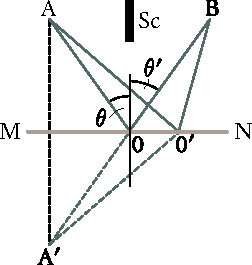
\includegraphics[scale=1]{figures/ch_16/fig_16_7.pdf}
% 		\caption[]{}
%         % \caption[]{Reflection and refraction of light using Fermat's principle.}
% 		\label{fig:16_7}
% 	\end{center}
% 	\vspace{-0.8cm}
% \end{figure}

Bây giờ ta sẽ tìm điểm mà tia sáng đi từ A đến B phải khúc xạ để quang trình đạt cực trị (\fig{16_8}).
Quang trình của một tia sáng bất kì là
\begin{equation*}
    L = n_1 s_1 + n_2 s_2 + n_1 \sqrt{a_1^2 + x^2} + n_2 \sqrt{a_2^2 + (b - x)^2}.
\end{equation*}

\noindent
Để tìm cực trị, ta đạo hàm $L$ theo $x$ rồi cho đạo hàm bằng không:
\begin{equation*}
    \diff{L}{x} = \frac{n_1 x}{\sqrt{a_1^2 + x^2}} - \frac{n_2 (b - x)}{\sqrt{a_2^2 + (b - x)^2}} = n_1 \frac{x}{s_1} - n_2 \frac{(b-x)}{s_2} = 0.
\end{equation*}

\noindent
Các hệ số của $n_1$ và $n_2$ lần lượt bằng $\sin\theta$ và $\sin\theta''$.
Do đó ta có quan hệ
\begin{equation*}
    n_1 \sin\theta = n_2 \sin\theta'',
\end{equation*}

\noindent
biểu diễn định luật khúc xạ ánh sáng [xem \eqn{16_26}].

Ta hãy xem xét sự phản xạ ở mặt trong của một ellipsoid tròn xoay (\fig{16_9}; $F_1$ và $F_2$ là các tiêu điểm của ellipsoid).
Theo định nghĩa của ellipse, các đường $F_10F_2$, $F_10'F_2$, $F_10''F_2$, etc. có độ dài bằng nhau.
Do đó, tất cả các tia sáng từ tiêu điểm $F_1$ phản xạ trên bề mặt rồi đến tiêu điểm $F_2$ là đẳng thời.
Trong trường hợp này, quang trình có giá trị dừng.
Nếu ta thay mặt ellipsoid bằng mặt MM có độ cong nhỏ hơn và được định hướng sao cho một tia sáng đi từ điểm $F_1$ đến điểm $F_2$ sau khi phản xạ trên MM, thì quãng đường $F_10F_1$ sẽ là cực tiểu.
Với mặt NN có độ cong lớn hơn ellipsoid, thì quãng đường $F_10F_2$ sẽ là cực đại.

\begin{figure}[!htb]
	\begin{minipage}[t]{0.48\linewidth}
		\begin{center}
			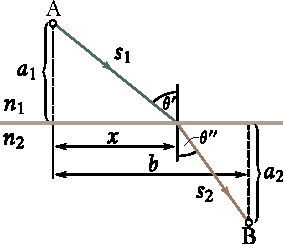
\includegraphics[scale=1]{figures/ch_16/fig_16_8.pdf}
			\caption[]{}
            % \caption[]{Ray travelling from A to B and refracted at the interface between $n_1$ and $n_2$.}
			\label{fig:16_8}
		\end{center}
	\end{minipage}
	\hfill{ }%space{-0.05cm}
	\begin{minipage}[t]{0.48\linewidth}
		\begin{center}
			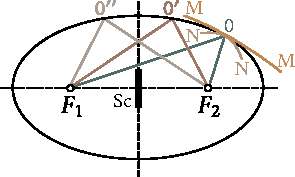
\includegraphics[scale=1]{figures/ch_16/fig_16_9.pdf}
            \caption[]{}
			% \caption[]{Reflection from the inner surface of an ellipsoid of revolution.}
			\label{fig:16_9}
		\end{center}
	\end{minipage}
\vspace{-0.4cm}
\end{figure}

Các quang trình cũng đạt giá trị dừng khi các tia sáng truyền qua một thấu kính (\fig{16_10}).
Trong tất cả các tia, thì tia P$0$P$'$ truyền quãng đường ngắn nhất trong không khí (môi trường có chiết suất $n$ bằng một đơn vị) và quãng đường dài nhất trong thủy tinh ($n\sim 1.5$).
Tia PQQ$'$P$'$ truyền quãng đường trong không khí dài nhất, nhưng lại truyền quãng đường ngắn hơn trong thủy tinh.
Kết quả là, quang trình của mọi tia sáng là như nhau.
Do đó, các tia sáng là đẳng thời, và quang trình đạt giá trị dừng.

Hãy xem xét sóng truyền theo các tia $1$, $2$, $3$,... trong một môi trường đẳng hướng không đồng nhất (\fig{16_11}).
Ta sẽ coi độ không đồng nhất là đủ nhỏ để có thể coi chiết suất là hằng số trên một đoạn tia sáng có độ dài $\lambda$.
Ta sẽ xây dựng các mặt sóng S$_1$, S$_2$, S$_3$,..., sao cho các dao động ở mỗi điểm của mặt sau trễ pha $2\pi$ so với các dao động tại mỗi điểm ở mặt liền trước.
Các dao động tại các điểm trên cùng tia sáng được mô tả bởi phương trình $\xi=A\cos(\omega t - kr + \alpha)$ (ở đây, $r$ là khoảng cách đo theo phương tia sáng).
Độ trễ pha được xác định bởi biểu thức $k\Delta{r}$, với $\Delta{r}$ là khoảng cách giữa các mặt liền kề.
Từ điều kiện $k\Delta{r}=2\pi$, ta tìm được $\Delta{r}=2\pi/k=\lambda$.
Quang trình của mỗi đoạn có độ dài hình học $\lambda$ là $n\lambda=\lambda_0$ [xem \eqn{16_5}].
Theo \eqn{16_54}, thời gian $\tau$ để tia sáng truyền hết một quãng đường tỉ lệ với quang trình của quãng đường đó.
Do đó, sự bằng nhau của các quang trình cho thấy sự bằng nhau của thời gian mà ánh sáng cần để đi hết các quãng đường tương ứng.
Vì vậy chúng ta đi đến kết luận rằng các phần tia sáng giới hạn giữa hai mặt sóng có quang trình bằng nhau và có tính đẳng thời.
Đặc biệt, các phần của các tia sáng giữa hai mặt sóng MM và NN mô tả bằng nét đứt trong \fig{16_10} là đẳng thời.

\begin{figure}[!htb]
	\begin{minipage}[t]{0.48\linewidth}
		\begin{center}
			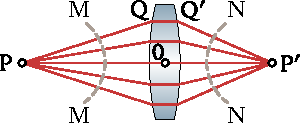
\includegraphics[scale=1]{figures/ch_16/fig_16_10.pdf}
			\caption[]{}
            % \caption[]{Stationary optical paths when light rays pass through a lens.}
			\label{fig:16_10}
		\end{center}
	\end{minipage}
	\hfill{ }%space{-0.05cm}
	\begin{minipage}[t]{0.48\linewidth}
		\begin{center}
			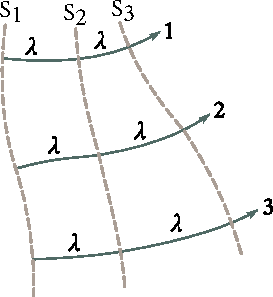
\includegraphics[scale=1]{figures/ch_16/fig_16_11.pdf}
            \caption[]{}
			% \caption[]{Wave propagating in a non-homogeneous isotropic medium along rays $1$, $2$, $3$.}
			\label{fig:16_11}
		\end{center}
	\end{minipage}
\vspace{-0.4cm}
\end{figure}

Từ những xử lý trên có thế thấy độ trễ pha $\delta$ xuất hiện trong quang trình $L$ được xác định bởi biểu thức
\begin{equation}\label{eq:16_55}
    \delta = \frac{L}{\lambda_0} 2\pi
\end{equation}

\noindent
($\lambda_0$ là bước sóng trong chân không).

\section{Hệ quang học trực tâm}\label{sec:16_7}

Một tập hợp các tia sáng tạo nên một chùm sáng.
Nếu các tia sáng giao nhau tại một điểm, thì chùm tia được gọi là đồng quy
Một mặt sóng cầu tương ứng với một chùm tia đồng quy.
Trên \ref{fig:16_12}a là chùm tia hội tụ, và trên \fig{16_12}b là một chùm phân kì.
Một trường hợp đặc biệt của chùm tia đồng quy là một chùm tia song song; tương ứng với một sóng ánh sáng phẳng.

Hệ quang học làm biến đổi các chùm sáng.
Nếu hệ không phá vỡ sự đồng quy của chùm sáng thì các tia sáng phát ra từ điểm P sẽ giao nhau tại một điểm P$'$.
Điểm này là \textbf{ảnh quang học} của điểm P. If a point of an object is depicted in the form of a point, the image is called a \textbf{point} or a \textbf{stigmatic} one (Nếu một điểm của vật cho ảnh dưới dạng một điểm, thì ảnh đó được gọi là một ảnh điểm hay một ảnh tương điểm).

Một ảnh được gọi là \textbf{thật} nếu các tia sáng thực sự cắt nhau tại điểm P$'$ (xem \fig{16_12}a), và \textbf{ảo} nếu đường kéo dài của các tia sáng (ngược với chiều truyền sáng) cắt nhau tại điểm P$'$ (xem \fig{16_12}b).

\begin{figure}[t]
	\begin{center}
		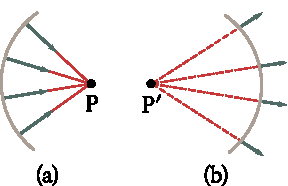
\includegraphics[scale=1]{figures/ch_16/fig_16_12.pdf}
		% \caption[]{Converging (a) and diverging (b) homocentric beam.}
        \caption[]{}
		\label{fig:16_12}
	\end{center}
	\vspace{-0.8cm}
\end{figure}

Do tính thuận nghịch của ánh sáng, nguồn sáng P và ảnh P$'$có thể hoán đổi vai trò cho nhau---một nguồn sáng đặt tại P$'$ sẽ cho ảnh tại P.
Vì vậy, P và P$'$ được gọi là các \textbf{điểm liên hợp}.

Một hệ quang học cho ra một ảnh quang học giống với vật về mặt hình học được gọi là hệ \textbf{lý tưởng}.
Với những hệ như vậy, sự liên tục trong không gian của các điểm P được mô tả dưới dạng sự liên tục trong không gian của các điểm P$'$.
Sự liên tục thứ nhất được gọi là \textbf{không gian vật}, và sự liên tục thứ hai được gọi là \textbf{không gian ảnh}.
Trong cả hai không gian, các điểm, đường thẳng và mặt phẳng là tương ứng duy nhất với nhau.
Quan hệ như vậy giữa hai không gian được gọi là \textbf{tương ứng cộng tuyến} trong hình học.

Một hệ quang học là một tập hợp các bề mặt phản xạ và khúc xạ được phân cách với nhau bởi các môi trường đồng nhất về mặt quang học.
Các mặt này thường là mặt cầu hoặc mặt phẳng (một mặt phẳng có thể được coi là một mặt cầu có bán kính bằng vô cùng).
Các mặt phức tạp hơn như ellipsoid, hyperboloid hay paraboloid tròn xoay ít được sử dụng đến hơn.

Một hệ quang học tạo bởi các mặt cầu (tính cả trường hợp đặc biệt là mặt phẳng) được gọi là \textbf{trực tâm} nếu tâm của tất cả các bề mặt đều nằm trên một đường thẳng duy nhất.
Đường thẳng này được gọi là \textbf{quang trục} của hệ.
Với mỗi điểm P hoặc mặt phẳng S trong không gian vật, tồn tại điểm liên hợp P$'$ hoặc mặt phẳng S$'$ tương ứng với nó trong không gian ảnh.
Một số lượng lớn đến vô cùng các điểm liên hợp và mặt phẳng liên hợp là các điểm và các mặt phẳng có những tính chất đặc biệt.
Các điểm và các mặt phẳng như vậy được gọi là \textbf{cơ điểm} hay \textbf{mặt phẳng cơ điểm}.
Các đối tượng như vậy bao gồm các điểm và mặt phẳng được gọi là \textbf{(mặt phẳng) tiêu điểm}, \textbf{(mặt phẳng) điểm chính}, và \textbf{(mặt phẳng) điểm nút}.
Bố trí của các điểm cardinal xác định đầy đủ các tính chất của một hệ quang học trực tâm lý tưởng.

\textbf{Tiêu diện và tiêu điểm của hệ quang học.}
Hình \ref{fig:16_13} thể hiện các mặt khúc xạ ngoài và quang trục của một hệ trực tâm lý tưởng.
Lấy mặt phẳng S vuông góc với quang trục trong không gian vật của hệ.
Xem xét đối xứng cho thấy mặt phẳng S$'$ liên hợp với S cũng vuông góc với quang trục.
Sự dịch chuyển của mặt phẳng S so với hệ sẽ gây ra sự dịch chuyển tương ứng của mặt phẳng S$'$.
Khi mặt phẳng S ở rất xa, thì việc dịch nó ra xa hệ hơn cũng không gây ra sự thay đổi vị trí đáng kể của mặt phẳng S$'$.
Điều này ngụ ý rằng khi dịch mặt phẳng S ra đến vô cùng, thì mặt phẳng S$'$ sẽ tiến đến một vị trí cực trị xác định F$'$. Mặt phẳng F$'$ trừng với vị trí của mặt phẳng S$'$ được gọi là \textbf{tiêu diện thứ hai} (hay \textbf{tiêu diện sau}) của quang hệ.
Ta có thể nói ngắn gọn rằng tiêu diện thứ hai F$'$ được định nghĩa là mặt phẳng liên hợp với mặt phẳng S$_{\infty}$ vuông góc với quang trục và đặt tại vô cùng trong không gian vật.

\begin{figure}[!htb]
	\begin{center}
		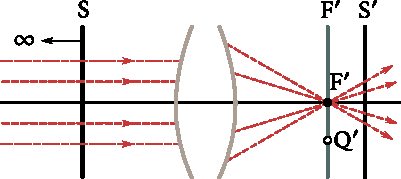
\includegraphics[scale=1]{figures/ch_16/fig_16_13.pdf}
		% \caption[]{External refracting surfaces and the optical axis of an ideal centered optical system. (Second focal point).}
        \caption[]{}
		\label{fig:16_13}
	\end{center}
	\vspace{-0.8cm}
\end{figure}

Giao điểm tiêu diện sau với quang trục được gọi là \textbf{tiêu điểm thứu hai} (hay \textbf{tiêu điểm sau}) của hệ.
Điểm này cũng được kí hiệu bằng chữ F$'$.
Điểm này là điểm liên hợp với P$_{\infty}$ ở vô cùng trên trục của hệ.
Các tia sáng xuất phát từ điểm P$_{\infty}$ sẽ tạo một chùm tia song song với trục (xem \fig{16_13}).
Khi các tia này ra khỏi hệ, chúng sẽ hội tụ tại tiêu điểm F$'$.
Một chùm sáng song song chiếu đến hệ cũng có thể không rời hệ dưới dạng một chùm tia hội tụ mà thay vào đó là dưới dạng một chùm phân kì (như \fig{16_13}).
Khi đó, điểm F$'$ không phải là giao điểm của các tia thực mà là giao điểm của các đường kéo dài theo hướng ngược với hướng tia sáng.
Vì vậy, tiêu diện thứ hai có thể ở trước quang hệ (theo hướng tia sáng) hoặc ở trong quang hệ.

Các tia phát ra từ điểm Q$_{\infty}$ ở xa vô cùng, không nằm trên quang trục sẽ tạo ra một chùm tia song song hợp một góc so với quang trục.
Sau khi ra khỏi hệ, những tia này tạo ra một chùm tia hội tụ tại điểm Q$'$ nằm trên tiêu diện thứ hai, nhưng không trùng với điểm F$'$ (xem điểm Q$'$ trong \fig{16_13}).
Từ đó ta thấy rằng ảnh của một vật đặt tại vô cùng sẽ nằm ở tiêu diện.

Nếu ta dịch mặt phẳng S$'$ vuông góc với trục ra vô cùng (\fig{16_14}), mặt phẳng liên hợp S sẽ dịch đến vị trí cực trị F được gọi là \textbf{tiêu diện thứ nhất} (hay \textbf{tiêu diện trước}) của hệ.
Có thể nói ngắn gọn rằng mặt phẳng F lằ mặt phẳng liên hợp với mặt phẳng S$_{\infty}'$ vuông góc với quang trục và đặt tại vô cùng trong không gian ảnh.

\begin{figure}[t]
	\begin{center}
		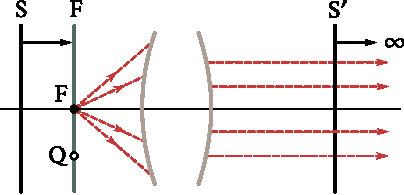
\includegraphics[scale=1]{figures/ch_16/fig_16_14.pdf}
		% \caption[]{External refracting surfaces and the optical axis of an ideal centered optical system. (First focal point).}
        \caption[]{}
		\label{fig:16_14}
	\end{center}
	\vspace{-0.8cm}
\end{figure}

Giao điểm của tiêu diện thứ nhất với quang trục được gọi là \textbf{tiêu điểm thứ nhất} (hay \textbf{tiêu điểm trước}) của hệ.
Điểm này cũng được kí hiệu bằng chữ F.
Các tia xuất phát từ tiêu điểm F sẽ tạo ra chùm tia ló song song với trục khi ra khỏi hệ. Các tia xuất phát từ điểm Q nằm trên tiêu diện F (xem \fig{16_14}) sau khi ra khỏi hệ sẽ tạo thành chùm tia ló song song tạo với quang trục một góc nào đó.
Cũng có thể chùm tia ló song song sau khi ra khỏi hệ được tạo ra từ chùm tia tới hội tụ, thay vì phân kì (như trong \fig{16_14}).
Trong trường hợp này, tiêu điểm thứ nhất có thể nằm trước hệ hoặc bên trong hệ.

\textbf{Các mặt phẳng chính và điểm chính.}
Ta xét hai mặt phẳng liên hợp vuông góc với quang trục của hệ.
Mũi tên $y$ (\fig{16_15}) ở mặt phẳng này sẽ cho ảnh là mũi tên $y'$ trong mặt phẳng còn lại.
Đối xứng trục của hệ cho thấy các mũi tên $y$ và $y'$ phải nằm trên cùng một mặt phẳng đi qua quang trục (trong mặt phẳng hình vẽ).
Ảnh $y'$ có thể cùng chiều với vật $y$ (xem \fig{16_15}a), hoặc ngược chiều với vật (xem \fig{16_15}b).
Trong trường hợp thứ nhất, ảnh được gọi là \textbf{dựng xuôi}, và trong trường hợp hai---\textbf{đảo ngược}.
Độ dài của các đoạn thẳng phía trên quang trục được coi là có độ dài dương, còn của những đoạn thẳng nằm dưới quang trục được coi là âm.
Độ dài thực của các đoạn thẳng được chỉ ra trong hình vẽ, các đại lượng $y$ và $-y'$ là dương.

\begin{figure}[!htb]
	\begin{center}
		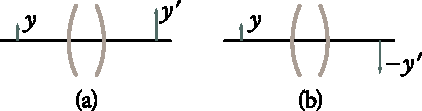
\includegraphics[scale=1]{figures/ch_16/fig_16_15.pdf}
		% \caption[]{Conjugate planes at right angles to the optical axis of the system. The image $y'$ may be in the same direction as object $y$ (a), or in the opposite direction (b).}
        \caption[]{}
		\label{fig:16_15}
	\end{center}
	\vspace{-0.8cm}
\end{figure}

Tỉ số của các kích thước dài giữa ảnh và vật được gọi là \textbf{độ phóng đại tuyến tính (độ phóng đại dài)} hay  \textbf{độ phóng đại ngang}.
Kí hiệu đại lượng đó bằng chữ $M$, ta có thể viết
\begin{equation}\label{eq:16_56}
    M = \frac{y'}{y}.
\end{equation}

\noindent
Độ phóng đại dài là một đại lượng đại số.
Nó nhận giá trị dương nếu ảnh xuôi chiều so với vật (dấu của $y$ và $y'$ giống nhau) và nhận giá trị âm nếu ảnh ngược chiều so với vật (dấu của $y$ và $y'$ ngược nhau).

Chúng ta có thể chứng minh rằng có hai mặt phẳng liên hợp phản xạ lẫn nhau với độ phóng đại tuyến tính là $M=+1$.
Các mặt phẳng này được gọi là các \textbf{mặt phẳng chính}.
Mặt phẳng chính thuộc không gian vật được gọi là mặt phẳng chính \textbf{thứ nhất} hay mặt phẳng chính \textbf{trước} của hệ.
Nó được kí hiệu là H. Mặt phẳng chính thuộc không gian ảnh được gọi là mặt phẳng chính \textbf{thứ hai} hay mặt phẳng chính \textbf{sau} của hệ.
Kí hiệu của nó là H$'$.
Các giao điểm của các mặt phẳng chính với quang trục được gọi là các \textbf{điểm chính} (thứ nhất và thứ hai) của hệ.
Chúng cũng được kí hiệu là H và H$'$.
Tùy thuộc vào thiết kế của hệ mà các điểm chính và mặt phẳng chính của nó có thể nằm trong hoặc ngoài hệ.
Một mặt phẳng chính có thể nằm ngoài hệ trong khi mặt phẳng còn lại nằm trong hệ.
Cuối cùng, cả hai mặt phẳng chính có thể cùng nằm ngoài và về mọt phía của hệ.

Từ định nghĩa của mặt phẳng chính có thể thấy rằng tia $1$ giao với mặt phẳng chính thứ nhất H tại điểm Q (thật---\fig{16_16}a, hay ảo do đường kéo dài vào trong hệ---\fig{16_16}b) có tia liên hợp $1'$ cắt mặt phẳng chính thứ hai H$'$ tại điểm Q$'$ (trực tiếp hay do đường kéo dài). Các điểm Q và Q$'$ nằm cùng phía so với quang trục và cách quang trục các khoảng bằng nhau.
Điều này là dễ hiểu nếu ta nhớ rằng Q và Q$'$ là hai điểm liên hợp, và mọi tia đi qua điểm Q thì cũng phải có một tia liên hợp đi qua điểm Q$'$.

\begin{figure}[!htb]
	\begin{center}
		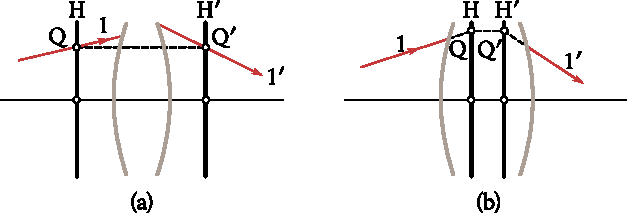
\includegraphics[scale=1]{figures/ch_16/fig_16_16h.pdf}
		% \caption[]{Conjugate points of the system intersecting principal planes.}
        \caption[]{}
		\label{fig:16_16}
	\end{center}
	\vspace{-0.7cm}
\end{figure}

\textbf{Mặt phẳng nút và điểm nút.}
Các điểm liên hợp N và N' nằm trên quang trục sao cho các tia liên hợp đi qua (hoặc có đường kéo dài đi qua) chúng song song với nhau được gọi là \textbf{các điểm nút} hay \textbf{nút} (xem các tia $1$-$1'$ và $2$-$2'$ trong \fig{16_17}).
Các mặt phẳng vuông góc với quang trục và đi qua các điểm nút được gọi là các \textbf{mặt phẳng nút} (thứ nhất và thứ hai).

Khoảng cách giữa các điểm nút luôn bằng khoảng cách giữa các điểm chính.
Khi các tính chất quang học của các môi trường ở hai phía hệ là giống nhau (tức là, $n = n'$), thì các điểm nút trùng với các điểm chính.

\begin{figure}[!htb]
	\begin{center}
		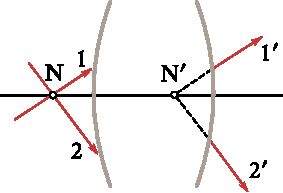
\includegraphics[scale=1]{figures/ch_16/fig_16_17.pdf}
		% \caption[]{Conjugate points N and N' lying on the optical axis.}
        \caption[]{}
		\label{fig:16_17}
	\end{center}
	\vspace{-0.8cm}
\end{figure}

\textbf{Tiêu cự và độ tụ của hệ.}
Khoảng cách từ điểm chính thứ nhất H đến tiêu cự thứ nhất F được gọi là \textbf{tiêu cự thứ nhất} $f$ của hệ.
Khoảng cách từ H' đến F' được gọi là \textbf{tiêu cự thứ hai} $f'$.
Các tiêu cự $f$ và $f'$, là các đại lượng đại số.
Chúng nhận giá trị dương nếu tiêu điểm đó nằm bên phải điểm chính tương ứng, và nhận giá trị âm trong trường hợp ngược lại.
Ví dụ, với hệ trong \fig{16_18} (xem bên dưới), tiêu cự thứ hai $f'$ là dương, còn tiêu cự thứ nhất $f$ là âm.
Hình vẽ biểu diễn độ dài thực của HF, tức là đại lượng dương (-$f$), bằng với giá trị tuyệt đối của $f$.

Ta có thể chỉ ra rằng giữa các tiêu cự $f$ và $f'$ của một hệ quang học trực tâm tạo bởi các mặt cầu khúc xạ có mối quan hệ:
\vspace{-12pt}
\begin{equation}\label{eq:16_57}
    \frac{f}{f'} = -\frac{n}{n'},
\end{equation}

\noindent
trong đó $n$ là chiết suất của môi trường phái trước hệ, và $n'$ là chiết suất của môi trường phía sau hệ.
Đánh giá \eqn{16_57} cho thấy khi chiết suất của các môi trường ở hai phái của quang hệ là như nhau, thì các tiêu cự chỉ khác nhau về dấu:
\begin{equation}\label{eq:16_58}
    f' = -f.
\end{equation}

Đại lượng
\begin{equation}\label{eq:16_59}
    P = \frac{n'}{f'} = - \frac{n}{f},
\end{equation}

\noindent
được gọi là \textbf{độ tụ} của một hệ.
Khi $P$ ngày càng tăng thì tiêu cự $f'$ ngày càng giảm, và do đó, the các tia sáng sẽ bị khúc xạ mạnh hơn khi đi qua quang hệ.
Độ tụ được đo bằng dioptre (D), khi đó, tiêu cự trong \eqn{16_59} phải được tính bằng mét.
Khi $P$ dương thì tiêu cự thứ hai $f'$ cũng dương; do đó, một điểm ở xa vô cùng sẽ có ảnh thật tạo bởi hệ---một chùm tia song song được biến đổi thành một chùm tia hội tụ.
Trong trường hợp này, hệ được gọi là \textbf{hệ hội tụ}.
Khi $P$ âm, ảnh của một điểm ở xa vô cùng sẽ là ảnh ảo---một chùm tia song song bị biến đổi thành một chùm tia phân kì bởi hệ. Hệ như vậy được gọi là \textbf{hệ phân kì}.

\begin{figure}[!htb]
	\begin{center}
		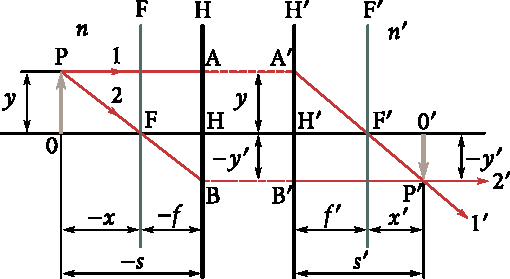
\includegraphics[scale=1]{figures/ch_16/fig_16_18.pdf}
		% \caption[]{Focal length of an optical system: the second focal length $f'$ is positive and the first focal length $f$ is negative.}
        \caption[]{}
		\label{fig:16_18}
	\end{center}
	\vspace{-0.8cm}
\end{figure}

\textbf{Công thức của hệ.}
Chúng ta xác định được đầy đủ các tính chất của một quang hệ nếu biết vị trí các cơ điểm và mặt phẳng cơ điểm của hệ đó.
Đặc biệt, khi đó ta còn có thể dựng ảnh quang học tạo bởi hệ.
Lấy đoạn thẳng OP vuông góc với quang trục trong không gian vật (\fig{16_18}, các điểm nút không được thể hiện trong hình). Vị trí củ đoạn thẳng này có thể được xác định bằng khoảng cách $x$ tính từ điểm F đến điểm $0$, hoặc bằng khoảng cách $s$ tính từ H đến $0$.
Các đại lượng $x$ và $s$, giống như các tiêu cự $f$ và $f'$, là các đại lượng đại số (độ lớn của chúng được ghi trên hình).

Ta vẽ tia sáng $1$ song song với quang trục, xuất phát từ điểm P.
Nó sẽ giao với mặt phẳng H ở điểm A.
Theo tính chất của các mặt phẳng chính, tia $1'$ liên hợp với tia $1$ phải đi qua điểm liên hợp với điểm A là A$'$ trên mặt phẳng H$'$.
Vì tia $1$ song song với quang trục, nên tia $1'$ liên hợp với nó sẽ đi qua tiêu điểm thứ hai F$'$.
Bây giờ ta vẽ tia $2$ xuất phát từ điểm P và đi qua tiêu điểm thứ nhất F.
Nó sẽ giao mặt phẳng H ở điểm B.
Tia $2'$ liên hợp với nó sẽ đi song song với quang trục và đi qua điểm liên hợp với B là điểm B$'$ trên mặt phẳng H$'$.
Điểm P$'$ giao giữa tia $1'$ và tia $2'$ là ảnh của điểm P.
Ảnh $0'$P$'$, cũng giống vật OP, đều vuông góc với quang trục.

Vị trí của ảnh $0'$P$'$ có thể được đặc trưng bởi khoảng cách $x'$ từ điểm F$'$ đến điểm $0'$ hoặc khoảng cách $s'$ từ H$'$ đến $0'$.
Các đại lượng $x'$ và $s'$ là các đại lượng đại số.
Trong trường hợp thể hiện ở \fig{16_18}, các đại lượng trên mang dấu dương.

Đại lượng $x'$ xác định vị trí của ảnh có sự liên hệ với đại lượng $x$ xác định vị trí của vật và với các tiêu cự $f$ và $f'$.
Với các tam giác vuông có đỉnh F chung (xem \fig{16_18}), ta có thể viết mối liên hệ:
\begin{equation}\label{eq:16_60}
    \frac{\text{OP}}{\text{HB}} = \frac{y}{-y'} = \frac{-x}{-f}.
\end{equation}

\noindent
Tương tự, với các tam giác có đỉnh F$'$ chung, ta có
\begin{equation}\label{eq:16_61}
    \frac{\text{H$'$A$'$}}{\text{O$'$P$'$}} = \frac{y}{-y'} = \frac{f'}{x'}.
\end{equation}

\noindent
Kết hợp hai hệ thức trên, ta thấy rằng $(-x)/(-f)=f'/x'$, hay
\begin{equation}\label{eq:16_62}
    xx' = ff'.
\end{equation}

\noindent
Phương trình này còn được gọi là \textbf{Công thức Newton}.
Trong điều kiện $n = n'$, công thức Newton có dạng
\begin{equation}\label{eq:16_63}
    xx' = -f^2
\end{equation}

\noindent
[xem \eqn{16_57}].

Ta có thể dễ dàng chuyển công thức liên hệ các khoảng cách $x$ từ vật và $x'$ từ ảnh đến tiêu điểm sang công thức liên hệ các khoảng cách $s$ từ vật và $s'$ từ ảnh đến điểm chính.
\fig{16_18} cho thấy $(-x) = (-s) - (-f)$ (tức là, $x=s-f$), và $x'=s'-f'$.
Thay các biểu thức này của $x$ và $x'$ vào \eqn{16_62} và biến đổi, ta thu được
\begin{equation}\label{eq:16_64}
    \frac{f}{s} + \frac{f'}{s'} = 1.
\end{equation}

\noindent
Trong điều kiện $f'=-f$ [xem \eqn{16_58}], \eqn{16_64} được đơn giản hóa thành:
\begin{equation}\label{eq:16_65}
    \frac{1}{s} - \frac{1}{s'} = \frac{1}{f}.
\end{equation}

\noindent
Các phương trình \eqref{eq:16_62}-\eqref{eq:16_65} là các phương trình của một hệ quang học đồng trục.

\section{Các thấu kính mỏng}\label{sec:16_8}

Một \textbf{thấu kính} là một hệ quang học trực tâm đơn giản.
Nó là một vật trong suốt (thường làm bằng thủy tinh) được giới hạn bởi hai mặt cầu\footnote{Cũng có những thấu kính có hình dạng bề mặt phức tạp hơn.} (đặc biệt có thấu kính có một mặt phẳng).
Các giao điểm của các mặt khúc xạ với quang trục được gọi là \textbf{đỉnh} của mặt đó.
Khoảng cách giữa các đỉnh được gọi là \textbf{độ dày} của thấu kính.
Nếu độ dày của thấu kính có thể bỏ qua so với bán kính cong của các mặt bao thấu kính thì thấu kính đó được gọi là \textbf{thấu kính mỏng}.

Các tính toán mà chúng ta sẽ không trình bày ở đây chỉ ra rằng các mặt phẳng chính H và H$'$ của thấu kính mỏng có thể coi là trùng nhau và cùng đi qua tâm $0$ của thấu kính (\fig{16_19}).
Ta nhận được biểu thức sau cho tiêu cự của một thấu kính mỏng:
\begin{equation}\label{eq:16_66}
    f' = -f = \parenthesis{\frac{n_0}{n-n_0}} \parenthesis{\frac{R_1R_2}{R_2-R_1}},
\end{equation}

\noindent
với $n$ là chiết suất của thấu kính, $n_0$ chiết suất của môi trường bao quanh thấu kính, $R_1$ và $R_2$ là các bán kính cong của các mặt thấu kính.

\begin{figure}[!htb]
	\begin{center}
		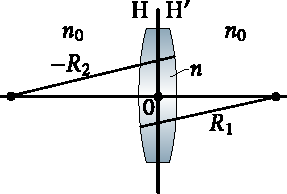
\includegraphics[scale=1]{figures/ch_16/fig_16_19.pdf}
		% \caption[]{Thin lens system: $n$ is the refractive index of the lens, $n_0$ is the refractive index of the medium surrounding the lens, $R_1$ and $R_2$ are the radii of curvature of the lens surfaces.}
        \caption[]{}
		\label{fig:16_19}
	\end{center}
	\vspace{-0.8cm}
\end{figure}

Ta sẽ bán kính cong như các đại lượng đại số: với mặt lồi (tức là, khi tâm cong nằm ở phía bên phải của đỉnh mặt cong) thì bán kính cong nhận giá trị dương, còn đối với một mặt lõm (tức là, khi tâm cong nằm bên trái đỉnh mặt cong) thì bán kính nhận giá trị âm.
Độ lớn của các bán kính cong được thể hiện trong hình vẽ, với $R < 0$ thì độ lớn là $-R$.

Nếu chiết suất của môi trường ở hai bên thấu kính mỏng là giống nhau, thì các điểm nút N và N$'$ trùng với các điểm chính, tức là , cùng nằm tại tâm $0$ của thấu kính.
Khi đó, mọi tia đi qua quang tâm của thấu kính đều không bị lệch hướng.
Nếu chiết suất của môi trường ở trước và sau thấu kính là khác nhau, thì các điểm nút không trùng với các điểm chính và một tia đi qua quang tâm của thấu kính sẽ bị lệch hướng.

Một chùm tia song song sau khi chiếu qua một thấu kính sẽ hội tụ tại một điểm trên tiêu diện (xem điểm Q$'$ trong \fig{16_20}).
Để xác định vị trí của điểm này, ta phải kéo dài tia đi qua quang tâm của thấu kính đến khi cắt tiêu diện (xem tia $0$Q$'$ được vẽ bằng nét đứt).
Các tia khác cũng sẽ đi qua giao điểm này.
phương pháp này thích hợp khi các tính chất quang học của các môi trường hai bên thấu kính là giống nhau ($n=n'$).
Nếu không, một tia đi qua quang tâm sẽ bị lệch hướng.
Để tìm điểm Q$'$ trong trường hợp này, ta phải biết vị trí các điểm nút của thấu kính.

Cần chú ý rằng quang trình của các tia xuất phát từ mặt sóng SS (xem \fig{16_20}) tới điểm Q$'$
là giống nhau và là đẳng thời (xem phần cuối \sect{16_6}).

Cuối cùng, phải chấp nhận rằng thấu kính không phải một hệ quang học lý tưởng.
Ảnh tạo bởi thấu kính có một số sai lệch.
Nhưng việc xem xét các sai lệch đó nằm ngoài phạm vi của cuốn sách này.

\begin{figure}[!htb]
	\begin{center}
		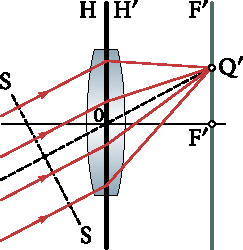
\includegraphics[scale=1]{figures/ch_16/fig_16_20.pdf}
		% \caption[]{Parallel beam of rays passign through a lens.}
        \caption[]{}
		\label{fig:16_20}
	\end{center}
	\vspace{-0.8cm}
\end{figure}

\section{Nguyên lý Huygens}\label{sec:16_9}

Trong hai chương tới, ta sẽ xem xét các hiện tượng diễn ra ở sau một màn chắn sáng khi sóng ánh sáng chiếu tới một lỗ nhỏ trên màn chắn đó.
Trong phép xấp sỉ của quang hình học, tia sáng không thể bị bẻ cong vào vùng bóng hình học.
Tuy nhiên, trong thực tế một sóng ánh sáng có thể lan truyền trong toàn bộ không gian phía sau màn chắn và bị bẻ cong vào vùng bóng quang học. Kích thước của lỗ càng nhỏ thì sự bẻ cong càng được thấy rõ.
Khi kích thước của lỗ vào cỡ bước sóng ánh sáng thì phép xấp xỉ quang hình học không còn hiệu lực nữa.

Hành vi của ánh sáng sau khi đi qua lỗ nhỏ trên màn chắn có thể được giải thích một cách định tính bằng \textbf{Nguyên lý Huygens}, đặt tên theo nhà vật lý người Hà Lan Christian Huygens (1629-1696), người khám phá ra nguyên lý này.
Nguyên lý này thiết lập cách xây dựng một mặt đầu sóng ở thời điểm $t+\Delta{t}$ từ vị trí đã biết của mặt đầu sóng ở thời điểm $t$.
Theo nguyên lý Huygens, mỗi điểm trên một mặt đầu sóng trước có thể được coi là một nguồn sóng thứ cấp, và đường bao của các sóng thứ cấp sẽ xác định mặt đầu sóng tiếp theo (\fig{16_21}; môi trường được giả sử là không đồng nhất---vận tốc của sóng ở phần dưới của hình lớn hơn ở phần trên của hình).

\begin{figure}[!htb]
	\begin{minipage}[t]{0.41\linewidth}
		\begin{center}
			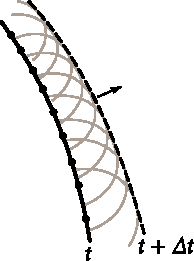
\includegraphics[scale=1]{figures/ch_16/fig_16_21.pdf}
			\caption[]{}
            % \caption[]{Huygens' principle: every point on an advancing wavefront can be considered as a source of secondary wavelets, and the envelope of these wavelets defines a new wavefront.}
			\label{fig:16_21}
		\end{center}
	\end{minipage}
	\hfill{ }%space{-0.05cm}
	\begin{minipage}[t]{0.55\linewidth}
		\begin{center}
			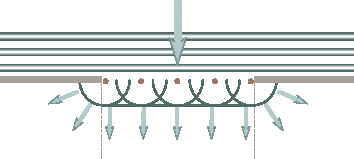
\includegraphics[scale=1]{figures/ch_16/fig_16_22.pdf}
            \caption[]{}
			% \caption[]{Huygens' diffraction: a plane barrier with an aperture is struck by a wavefront parallel to it. Every point on the portion of the wavefront bordering on the aperture is a centre of secondary wavelets which will be spherical in a homogeneous and isotropic medium.}
			\label{fig:16_22}
		\end{center}
	\end{minipage}
\vspace{-0.4cm}
\end{figure}

Giả sử một mặt đầu sóng song song với một màn chắn chiếu tới một lỗ nhỏ trên màn chắn đó (\fig{16_22}).
Theo Huygens, mỗi điểm trên mặt tiếp giáp giữa mặt sóng và lỗ là một nguồn sáng thứ cấp có dạng sóng cầu, giả sử môi trường là đồng nhất và đẳng hướng. Vẽ đường bao của các sóng thứ cấp đó ta sẽ thấy sóng uốn quanh cạnh của lỗ và bị bẻ cong vào vùng bóng quang học (nằm ngoài đường nét đứt ở phía sau màn chắn).

Nguyên lý Huygens không cho ta bất kì thông tin gì về cường độ của sóng truyền theo các hướng khác nhau.
Thiếu sót này đã được nhà vật lý người Pháp Augustin Fresnel (1788-1827) khắc phục.
Nguyên lý Huygens-Fresnel và các ví dụ vật lý được xem xét trong \sect{18_1}.
